\documentclass[twoside]{book}

% Packages required by doxygen
\usepackage{fixltx2e}
\usepackage{calc}
\usepackage{doxygen}
\usepackage[export]{adjustbox} % also loads graphicx
\usepackage{graphicx}
\usepackage[utf8]{inputenc}
\usepackage{makeidx}
\usepackage{multicol}
\usepackage{multirow}
\PassOptionsToPackage{warn}{textcomp}
\usepackage{textcomp}
\usepackage[nointegrals]{wasysym}
\usepackage[table]{xcolor}

% Font selection
\usepackage[T1]{fontenc}
\usepackage[scaled=.90]{helvet}
\usepackage{courier}
\usepackage{amssymb}
\usepackage{sectsty}
\renewcommand{\familydefault}{\sfdefault}
\allsectionsfont{%
  \fontseries{bc}\selectfont%
  \color{darkgray}%
}
\renewcommand{\DoxyLabelFont}{%
  \fontseries{bc}\selectfont%
  \color{darkgray}%
}
\newcommand{\+}{\discretionary{\mbox{\scriptsize$\hookleftarrow$}}{}{}}

% Page & text layout
\usepackage{geometry}
\geometry{%
  a4paper,%
  top=2.5cm,%
  bottom=2.5cm,%
  left=2.5cm,%
  right=2.5cm%
}
\tolerance=750
\hfuzz=15pt
\hbadness=750
\setlength{\emergencystretch}{15pt}
\setlength{\parindent}{0cm}
\setlength{\parskip}{3ex plus 2ex minus 2ex}
\makeatletter
\renewcommand{\paragraph}{%
  \@startsection{paragraph}{4}{0ex}{-1.0ex}{1.0ex}{%
    \normalfont\normalsize\bfseries\SS@parafont%
  }%
}
\renewcommand{\subparagraph}{%
  \@startsection{subparagraph}{5}{0ex}{-1.0ex}{1.0ex}{%
    \normalfont\normalsize\bfseries\SS@subparafont%
  }%
}
\makeatother

% Headers & footers
\usepackage{fancyhdr}
\pagestyle{fancyplain}
\fancyhead[LE]{\fancyplain{}{\bfseries\thepage}}
\fancyhead[CE]{\fancyplain{}{}}
\fancyhead[RE]{\fancyplain{}{\bfseries\leftmark}}
\fancyhead[LO]{\fancyplain{}{\bfseries\rightmark}}
\fancyhead[CO]{\fancyplain{}{}}
\fancyhead[RO]{\fancyplain{}{\bfseries\thepage}}
\fancyfoot[LE]{\fancyplain{}{}}
\fancyfoot[CE]{\fancyplain{}{}}
\fancyfoot[RE]{\fancyplain{}{\bfseries\scriptsize Generated by Doxygen }}
\fancyfoot[LO]{\fancyplain{}{\bfseries\scriptsize Generated by Doxygen }}
\fancyfoot[CO]{\fancyplain{}{}}
\fancyfoot[RO]{\fancyplain{}{}}
\renewcommand{\footrulewidth}{0.4pt}
\renewcommand{\chaptermark}[1]{%
  \markboth{#1}{}%
}
\renewcommand{\sectionmark}[1]{%
  \markright{\thesection\ #1}%
}

% Indices & bibliography
\usepackage{natbib}
\usepackage[titles]{tocloft}
\setcounter{tocdepth}{3}
\setcounter{secnumdepth}{5}
\makeindex

% Hyperlinks (required, but should be loaded last)
\usepackage{ifpdf}
\ifpdf
  \usepackage[pdftex,pagebackref=true]{hyperref}
\else
  \usepackage[ps2pdf,pagebackref=true]{hyperref}
\fi
\hypersetup{%
  colorlinks=true,%
  linkcolor=blue,%
  citecolor=blue,%
  unicode%
}

% Custom commands
\newcommand{\clearemptydoublepage}{%
  \newpage{\pagestyle{empty}\cleardoublepage}%
}

\usepackage{caption}
\captionsetup{labelsep=space,justification=centering,font={bf},singlelinecheck=off,skip=4pt,position=top}

%===== C O N T E N T S =====

\begin{document}

% Titlepage & ToC
\hypersetup{pageanchor=false,
             bookmarksnumbered=true,
             pdfencoding=unicode
            }
\pagenumbering{alph}
\begin{titlepage}
\vspace*{7cm}
\begin{center}%
{\Large My Project }\\
\vspace*{1cm}
{\large Generated by Doxygen 1.8.14}\\
\end{center}
\end{titlepage}
\clearemptydoublepage
\pagenumbering{roman}
\tableofcontents
\clearemptydoublepage
\pagenumbering{arabic}
\hypersetup{pageanchor=true}

%--- Begin generated contents ---
\chapter{Hierarchical Index}
\section{Class Hierarchy}
This inheritance list is sorted roughly, but not completely, alphabetically\+:\begin{DoxyCompactList}
\item \contentsline{section}{Atom}{\pageref{structAtom}}{}
\item \contentsline{section}{Container\+Base$<$ T $>$}{\pageref{structContainerBase}}{}
\item \contentsline{section}{Container\+Base$<$ std\+:\+:vector$<$ Atom $>$ $>$}{\pageref{structContainerBase}}{}
\begin{DoxyCompactList}
\item \contentsline{section}{Molecule}{\pageref{classMolecule}}{}
\end{DoxyCompactList}
\item \contentsline{section}{Container\+Base$<$ std\+:\+:vector$<$ Molecule $>$ $>$}{\pageref{structContainerBase}}{}
\begin{DoxyCompactList}
\item \contentsline{section}{Topology}{\pageref{classTopology}}{}
\end{DoxyCompactList}
\item \contentsline{section}{Container\+Base$<$ std\+:\+:vector$<$ std\+:\+:pair$<$ std\+:\+:size\+\_\+t, std\+:\+:size\+\_\+t $>$ $>$ $>$}{\pageref{structContainerBase}}{}
\begin{DoxyCompactList}
\item \contentsline{section}{Criterion\+Base}{\pageref{classCriterionBase}}{}
\begin{DoxyCompactList}
\item \contentsline{section}{Criterion\+Angle}{\pageref{classCriterionAngle}}{}
\item \contentsline{section}{Criterion\+Dihedral}{\pageref{classCriterionDihedral}}{}
\item \contentsline{section}{Criterion\+Distance}{\pageref{classCriterionDistance}}{}
\end{DoxyCompactList}
\end{DoxyCompactList}
\item \contentsline{section}{Controller}{\pageref{classController}}{}
\item \contentsline{section}{Energy\+Parser\+Base}{\pageref{classEnergyParserBase}}{}
\begin{DoxyCompactList}
\item \contentsline{section}{Energy\+Parser\+G\+MX}{\pageref{classEnergyParserGMX}}{}
\end{DoxyCompactList}
\item \contentsline{section}{Engine\+Base}{\pageref{classEngineBase}}{}
\begin{DoxyCompactList}
\item \contentsline{section}{Engine\+G\+MX}{\pageref{classEngineGMX}}{}
\end{DoxyCompactList}
\item \contentsline{section}{Parameters}{\pageref{classParameters}}{}
\item \contentsline{section}{Reaction\+Base}{\pageref{classReactionBase}}{}
\begin{DoxyCompactList}
\item \contentsline{section}{Reaction\+Candidate}{\pageref{classReactionCandidate}}{}
\end{DoxyCompactList}
\item \contentsline{section}{Reaction\+Parser}{\pageref{classReactionParser}}{}
\item \contentsline{section}{Simulator\+Base}{\pageref{classSimulatorBase}}{}
\begin{DoxyCompactList}
\item \contentsline{section}{Simulator\+Metropolis}{\pageref{classSimulatorMetropolis}}{}
\item \contentsline{section}{Simulator\+Rate}{\pageref{classSimulatorRate}}{}
\end{DoxyCompactList}
\item \contentsline{section}{Topology\+Parser\+Base}{\pageref{classTopologyParserBase}}{}
\begin{DoxyCompactList}
\item \contentsline{section}{Topology\+Parser\+G\+MX}{\pageref{classTopologyParserGMX}}{}
\end{DoxyCompactList}
\item \contentsline{section}{Transition\+Table}{\pageref{structTransitionTable}}{}
\item \contentsline{section}{Translation\+Table}{\pageref{structTranslationTable}}{}
\item \contentsline{section}{Universe}{\pageref{classUniverse}}{}
\item \contentsline{section}{enhance\+:\+:Vector3d$<$ T $>$}{\pageref{classenhance_1_1Vector3d}}{}
\end{DoxyCompactList}

\chapter{Class Index}
\section{Class List}
Here are the classes, structs, unions and interfaces with brief descriptions\+:\begin{DoxyCompactList}
\item\contentsline{section}{\mbox{\hyperlink{structAtom}{Atom}} }{\pageref{structAtom}}{}
\item\contentsline{section}{\mbox{\hyperlink{structContainerBase}{Container\+Base$<$ T $>$}} }{\pageref{structContainerBase}}{}
\item\contentsline{section}{\mbox{\hyperlink{classController}{Controller}} }{\pageref{classController}}{}
\item\contentsline{section}{\mbox{\hyperlink{classCriterionAngle}{Criterion\+Angle}} }{\pageref{classCriterionAngle}}{}
\item\contentsline{section}{\mbox{\hyperlink{classCriterionBase}{Criterion\+Base}} }{\pageref{classCriterionBase}}{}
\item\contentsline{section}{\mbox{\hyperlink{classCriterionDihedral}{Criterion\+Dihedral}} }{\pageref{classCriterionDihedral}}{}
\item\contentsline{section}{\mbox{\hyperlink{classCriterionDistance}{Criterion\+Distance}} }{\pageref{classCriterionDistance}}{}
\item\contentsline{section}{\mbox{\hyperlink{classEnergyParserBase}{Energy\+Parser\+Base}} }{\pageref{classEnergyParserBase}}{}
\item\contentsline{section}{\mbox{\hyperlink{classEnergyParserGMX}{Energy\+Parser\+G\+MX}} }{\pageref{classEnergyParserGMX}}{}
\item\contentsline{section}{\mbox{\hyperlink{classEngineBase}{Engine\+Base}} }{\pageref{classEngineBase}}{}
\item\contentsline{section}{\mbox{\hyperlink{classEngineGMX}{Engine\+G\+MX}} }{\pageref{classEngineGMX}}{}
\item\contentsline{section}{\mbox{\hyperlink{classMolecule}{Molecule}} }{\pageref{classMolecule}}{}
\item\contentsline{section}{\mbox{\hyperlink{classParameters}{Parameters}} }{\pageref{classParameters}}{}
\item\contentsline{section}{\mbox{\hyperlink{classReactionBase}{Reaction\+Base}} }{\pageref{classReactionBase}}{}
\item\contentsline{section}{\mbox{\hyperlink{classReactionCandidate}{Reaction\+Candidate}} }{\pageref{classReactionCandidate}}{}
\item\contentsline{section}{\mbox{\hyperlink{classReactionParser}{Reaction\+Parser}} }{\pageref{classReactionParser}}{}
\item\contentsline{section}{\mbox{\hyperlink{classSimulatorBase}{Simulator\+Base}} }{\pageref{classSimulatorBase}}{}
\item\contentsline{section}{\mbox{\hyperlink{classSimulatorMetropolis}{Simulator\+Metropolis}} }{\pageref{classSimulatorMetropolis}}{}
\item\contentsline{section}{\mbox{\hyperlink{classSimulatorRate}{Simulator\+Rate}} }{\pageref{classSimulatorRate}}{}
\item\contentsline{section}{\mbox{\hyperlink{classTopology}{Topology}} }{\pageref{classTopology}}{}
\item\contentsline{section}{\mbox{\hyperlink{classTopologyParserBase}{Topology\+Parser\+Base}} }{\pageref{classTopologyParserBase}}{}
\item\contentsline{section}{\mbox{\hyperlink{classTopologyParserGMX}{Topology\+Parser\+G\+MX}} }{\pageref{classTopologyParserGMX}}{}
\item\contentsline{section}{\mbox{\hyperlink{structTransitionTable}{Transition\+Table}} }{\pageref{structTransitionTable}}{}
\item\contentsline{section}{\mbox{\hyperlink{structTranslationTable}{Translation\+Table}} }{\pageref{structTranslationTable}}{}
\item\contentsline{section}{\mbox{\hyperlink{classUniverse}{Universe}} }{\pageref{classUniverse}}{}
\item\contentsline{section}{\mbox{\hyperlink{classenhance_1_1Vector3d}{enhance\+::\+Vector3d$<$ T $>$}} }{\pageref{classenhance_1_1Vector3d}}{}
\end{DoxyCompactList}

\chapter{Class Documentation}
\hypertarget{structAtom}{}\section{Atom Struct Reference}
\label{structAtom}\index{Atom@{Atom}}
\subsection*{Public Member Functions}
\begin{DoxyCompactItemize}
\item 
\mbox{\Hypertarget{structAtom_afdda6123eb6378f48a81d4860ba2f193}\label{structAtom_afdda6123eb6378f48a81d4860ba2f193}} 
bool {\bfseries operator==} (const \mbox{\hyperlink{structAtom}{Atom}} \&other) const
\item 
\mbox{\Hypertarget{structAtom_af989a0a832cb20ba634432a7bb5b1419}\label{structAtom_af989a0a832cb20ba634432a7bb5b1419}} 
bool {\bfseries operator!=} (const \mbox{\hyperlink{structAtom}{Atom}} \&other) const
\item 
\mbox{\Hypertarget{structAtom_a3bd520b3b4b590626ea3c9b285ef2bec}\label{structAtom_a3bd520b3b4b590626ea3c9b285ef2bec}} 
bool {\bfseries operator$<$} (const \mbox{\hyperlink{structAtom}{Atom}} \&other) const
\item 
\mbox{\Hypertarget{structAtom_a7c849476ba49a1eedd6a1309065ce2ff}\label{structAtom_a7c849476ba49a1eedd6a1309065ce2ff}} 
bool {\bfseries operator$>$} (const \mbox{\hyperlink{structAtom}{Atom}} \&other) const
\end{DoxyCompactItemize}
\subsection*{Public Attributes}
\begin{DoxyCompactItemize}
\item 
\mbox{\Hypertarget{structAtom_a5ac7dd8b24a3e438c2e19b1ca8e1b7c8}\label{structAtom_a5ac7dd8b24a3e438c2e19b1ca8e1b7c8}} 
std\+::size\+\_\+t {\bfseries id} \{0\}
\item 
\mbox{\Hypertarget{structAtom_a7ad8efbefc804cbff230750350283136}\label{structAtom_a7ad8efbefc804cbff230750350283136}} 
std\+::string {\bfseries name} \{\}
\item 
\mbox{\Hypertarget{structAtom_a482804d6dc561ba73a8d543b2e6eb450}\label{structAtom_a482804d6dc561ba73a8d543b2e6eb450}} 
R\+E\+A\+L\+V\+EC {\bfseries position} \{0, 0, 0\}
\item 
\mbox{\Hypertarget{structAtom_aee46bbc59f76f455219eb94367a6641b}\label{structAtom_aee46bbc59f76f455219eb94367a6641b}} 
R\+E\+A\+L\+V\+EC {\bfseries velocity} \{0, 0, 0\}
\end{DoxyCompactItemize}
\subsection*{Friends}
\begin{DoxyCompactItemize}
\item 
\mbox{\Hypertarget{structAtom_a0b4533cd3ad55d6afaba9d291ded714b}\label{structAtom_a0b4533cd3ad55d6afaba9d291ded714b}} 
std\+::ostream \& {\bfseries operator$<$$<$} (std\+::ostream \&, const \mbox{\hyperlink{structAtom}{Atom}} \&)
\end{DoxyCompactItemize}


The documentation for this struct was generated from the following file\+:\begin{DoxyCompactItemize}
\item 
container/atom.\+hpp\end{DoxyCompactItemize}

\hypertarget{structContainerBase}{}\section{Container\+Base$<$ T $>$ Struct Template Reference}
\label{structContainerBase}\index{Container\+Base$<$ T $>$@{Container\+Base$<$ T $>$}}
\subsection*{Public Member Functions}
\begin{DoxyCompactItemize}
\item 
\mbox{\Hypertarget{structContainerBase_a36863f426649fe209bdb8459861f77aa}\label{structContainerBase_a36863f426649fe209bdb8459861f77aa}} 
auto \& {\bfseries operator()} (std\+::size\+\_\+t i)
\item 
\mbox{\Hypertarget{structContainerBase_a6bd5fceec65901efbef4e4080e9b803a}\label{structContainerBase_a6bd5fceec65901efbef4e4080e9b803a}} 
constexpr auto \& {\bfseries operator()} (std\+::size\+\_\+t i) const
\item 
\mbox{\Hypertarget{structContainerBase_a97b23eefaf74d425031f4a6e38fb3e52}\label{structContainerBase_a97b23eefaf74d425031f4a6e38fb3e52}} 
auto \& {\bfseries operator\mbox{[}$\,$\mbox{]}} (std\+::size\+\_\+t i)
\item 
\mbox{\Hypertarget{structContainerBase_aedf8882ba2cccd9dd3913b50e1ab56e2}\label{structContainerBase_aedf8882ba2cccd9dd3913b50e1ab56e2}} 
constexpr auto \& {\bfseries operator\mbox{[}$\,$\mbox{]}} (std\+::size\+\_\+t i) const
\item 
\mbox{\Hypertarget{structContainerBase_a5b2e85411107281947091c419affa761}\label{structContainerBase_a5b2e85411107281947091c419affa761}} 
auto {\bfseries begin} ()
\item 
\mbox{\Hypertarget{structContainerBase_a33b0e3d4bda02de8dce699c1cb1813e6}\label{structContainerBase_a33b0e3d4bda02de8dce699c1cb1813e6}} 
auto {\bfseries end} ()
\item 
\mbox{\Hypertarget{structContainerBase_ade415cd17e3385d04188c28c673fe275}\label{structContainerBase_ade415cd17e3385d04188c28c673fe275}} 
auto {\bfseries begin} () const
\item 
\mbox{\Hypertarget{structContainerBase_a27bd2d66c75e7f9e387bced476105b37}\label{structContainerBase_a27bd2d66c75e7f9e387bced476105b37}} 
auto {\bfseries end} () const
\item 
\mbox{\Hypertarget{structContainerBase_aee5c1554129dc52b7ae87f411276b9fe}\label{structContainerBase_aee5c1554129dc52b7ae87f411276b9fe}} 
auto {\bfseries cbegin} () const
\item 
\mbox{\Hypertarget{structContainerBase_a2aeb1fa9fb43d5a2f11c4698ff14d88a}\label{structContainerBase_a2aeb1fa9fb43d5a2f11c4698ff14d88a}} 
auto {\bfseries cend} () const
\item 
\mbox{\Hypertarget{structContainerBase_addd173b48b92058c498c62e4a07b1c1c}\label{structContainerBase_addd173b48b92058c498c62e4a07b1c1c}} 
auto {\bfseries rbegin} ()
\item 
\mbox{\Hypertarget{structContainerBase_a07973ea9c9f0b2081ca5b9fc61d6d5e4}\label{structContainerBase_a07973ea9c9f0b2081ca5b9fc61d6d5e4}} 
auto {\bfseries rend} ()
\item 
\mbox{\Hypertarget{structContainerBase_aba04fc68e37cc08d6a60be5e6b7406bd}\label{structContainerBase_aba04fc68e37cc08d6a60be5e6b7406bd}} 
auto {\bfseries rbegin} () const
\item 
\mbox{\Hypertarget{structContainerBase_a4c800252a4a7f9c8ba726c63a6293b94}\label{structContainerBase_a4c800252a4a7f9c8ba726c63a6293b94}} 
auto {\bfseries rend} () const
\item 
\mbox{\Hypertarget{structContainerBase_acd4dd0a72272d2a87f11cba5f81edf17}\label{structContainerBase_acd4dd0a72272d2a87f11cba5f81edf17}} 
auto {\bfseries crbegin} () const
\item 
\mbox{\Hypertarget{structContainerBase_a1c9c324e8df266e5699339e2c8537e7b}\label{structContainerBase_a1c9c324e8df266e5699339e2c8537e7b}} 
auto {\bfseries crend} () const
\item 
\mbox{\Hypertarget{structContainerBase_a4a96296d6d7dc7a6c74f74004ac23b76}\label{structContainerBase_a4a96296d6d7dc7a6c74f74004ac23b76}} 
auto {\bfseries size} () const
\item 
\mbox{\Hypertarget{structContainerBase_aa1c4fad982768641f6cf0b6302cae84d}\label{structContainerBase_aa1c4fad982768641f6cf0b6302cae84d}} 
auto \& {\bfseries front} ()
\item 
\mbox{\Hypertarget{structContainerBase_a063224cd9e276464edecef14277e3441}\label{structContainerBase_a063224cd9e276464edecef14277e3441}} 
const auto \& {\bfseries front} () const
\item 
\mbox{\Hypertarget{structContainerBase_ade5123296bce89f760d438860d6129c4}\label{structContainerBase_ade5123296bce89f760d438860d6129c4}} 
auto \& {\bfseries back} ()
\item 
\mbox{\Hypertarget{structContainerBase_a27fbe00d5a1fb04a288c3f6ed4ba617b}\label{structContainerBase_a27fbe00d5a1fb04a288c3f6ed4ba617b}} 
const auto \& {\bfseries back} () const
\end{DoxyCompactItemize}
\subsection*{Public Attributes}
\begin{DoxyCompactItemize}
\item 
\mbox{\Hypertarget{structContainerBase_ad27f75d60f395b9405c21531f903e1dc}\label{structContainerBase_ad27f75d60f395b9405c21531f903e1dc}} 
T {\bfseries data} \{\}
\end{DoxyCompactItemize}


The documentation for this struct was generated from the following file\+:\begin{DoxyCompactItemize}
\item 
container/container\+Base.\+hpp\end{DoxyCompactItemize}

\hypertarget{classController}{}\section{Controller Class Reference}
\label{classController}\index{Controller@{Controller}}
\subsection*{Public Member Functions}
\begin{DoxyCompactItemize}
\item 
\mbox{\Hypertarget{classController_af3c733ac55b6e4240899c995dd92a4dd}\label{classController_af3c733ac55b6e4240899c995dd92a4dd}} 
void {\bfseries setup} (int argc, char $\ast$argv\mbox{[}$\,$\mbox{]})
\item 
\mbox{\Hypertarget{classController_ad535ad74055e645b7f44b7feeb4e82a8}\label{classController_ad535ad74055e645b7f44b7feeb4e82a8}} 
void {\bfseries start} ()
\item 
\mbox{\Hypertarget{classController_ad2abd6ee544cb1cb39705f31c6700f0c}\label{classController_ad2abd6ee544cb1cb39705f31c6700f0c}} 
void {\bfseries stop} ()
\end{DoxyCompactItemize}
\subsection*{Static Public Member Functions}
\begin{DoxyCompactItemize}
\item 
\mbox{\Hypertarget{classController_aea878ac8e8b3c0b90876efc898afe7e7}\label{classController_aea878ac8e8b3c0b90876efc898afe7e7}} 
static void {\bfseries signal} (int S\+IG)
\end{DoxyCompactItemize}
\subsection*{Static Public Attributes}
\begin{DoxyCompactItemize}
\item 
\mbox{\Hypertarget{classController_a60d49e6e7564d5c7de0d121a518adf21}\label{classController_a60d49e6e7564d5c7de0d121a518adf21}} 
static std\+::atomic$<$ int $>$ {\bfseries S\+I\+G\+N\+AL} = \{0\}
\item 
\mbox{\Hypertarget{classController_a0aea87001970ceb43f8cd3882df4beb5}\label{classController_a0aea87001970ceb43f8cd3882df4beb5}} 
static std\+::atomic$<$ bool $>$ {\bfseries C\+I\+V\+I\+L\+I\+S\+E\+D\+\_\+\+S\+H\+U\+T\+D\+O\+WN} = \{false\}
\end{DoxyCompactItemize}


The documentation for this class was generated from the following files\+:\begin{DoxyCompactItemize}
\item 
control/controller.\+hpp\item 
control/controller.\+cpp\end{DoxyCompactItemize}

\hypertarget{classCriterionAngle}{}\section{Criterion\+Angle Class Reference}
\label{classCriterionAngle}\index{Criterion\+Angle@{Criterion\+Angle}}
Inheritance diagram for Criterion\+Angle\+:\begin{figure}[H]
\begin{center}
\leavevmode
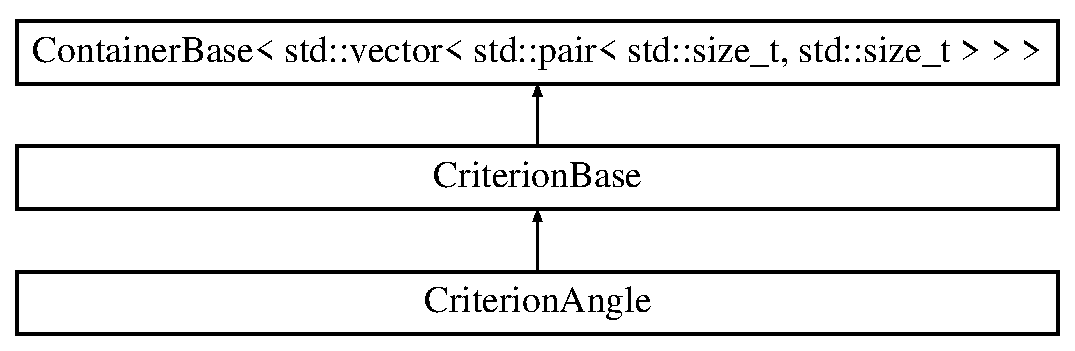
\includegraphics[height=3.000000cm]{classCriterionAngle}
\end{center}
\end{figure}
\subsection*{Public Member Functions}
\begin{DoxyCompactItemize}
\item 
\mbox{\Hypertarget{classCriterionAngle_ac549e87340ba17239eac219cad432853}\label{classCriterionAngle_ac549e87340ba17239eac219cad432853}} 
virtual std\+::string {\bfseries get\+Type} () const override
\item 
\mbox{\Hypertarget{classCriterionAngle_aaf0266c26e65098b6281d6f26cc47a74}\label{classCriterionAngle_aaf0266c26e65098b6281d6f26cc47a74}} 
bool {\bfseries valid} (const std\+::vector$<$ \mbox{\hyperlink{classMolecule}{Molecule}} $>$ \&reactants, const R\+E\+A\+L\+V\+EC \&box\+Dimensions)
\end{DoxyCompactItemize}
\subsection*{Protected Member Functions}
\begin{DoxyCompactItemize}
\item 
\mbox{\Hypertarget{classCriterionAngle_a66caa27b7ea5565bdd711e64b38225f2}\label{classCriterionAngle_a66caa27b7ea5565bdd711e64b38225f2}} 
virtual \mbox{\hyperlink{classCriterionAngle}{Criterion\+Angle}} $\ast$ {\bfseries clone\+\_\+impl} () const override
\end{DoxyCompactItemize}
\subsection*{Additional Inherited Members}


The documentation for this class was generated from the following file\+:\begin{DoxyCompactItemize}
\item 
reaction/criterion\+Derived.\+hpp\end{DoxyCompactItemize}

\hypertarget{classCriterionBase}{}\section{Criterion\+Base Class Reference}
\label{classCriterionBase}\index{Criterion\+Base@{Criterion\+Base}}
Inheritance diagram for Criterion\+Base\+:\begin{figure}[H]
\begin{center}
\leavevmode
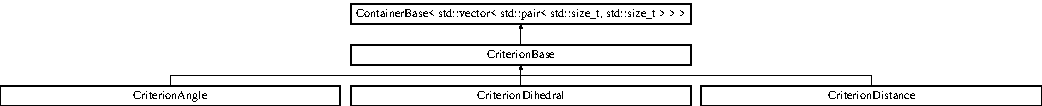
\includegraphics[height=1.421320cm]{classCriterionBase}
\end{center}
\end{figure}
\subsection*{Public Member Functions}
\begin{DoxyCompactItemize}
\item 
\mbox{\Hypertarget{classCriterionBase_a7bb6717dc8824634d0c240a077e534ad}\label{classCriterionBase_a7bb6717dc8824634d0c240a077e534ad}} 
virtual std\+::string {\bfseries get\+Type} () const =0
\item 
\mbox{\Hypertarget{classCriterionBase_af63fcfe2322e6592e1b0c52742c4dd7a}\label{classCriterionBase_af63fcfe2322e6592e1b0c52742c4dd7a}} 
void {\bfseries set\+Thresholds} (const R\+E\+AL \&min, const R\+E\+AL \&max)
\item 
\mbox{\Hypertarget{classCriterionBase_a74c8a877c6fa8bbb4138fb7ec4c054b3}\label{classCriterionBase_a74c8a877c6fa8bbb4138fb7ec4c054b3}} 
void {\bfseries set\+Thresholds} (const std\+::pair$<$ R\+E\+AL, R\+E\+AL $>$ \&values)
\item 
\mbox{\Hypertarget{classCriterionBase_a4253f38d43eb7be87df0743ac2c301d2}\label{classCriterionBase_a4253f38d43eb7be87df0743ac2c301d2}} 
void {\bfseries set\+Min} (const R\+E\+AL \&value)
\item 
\mbox{\Hypertarget{classCriterionBase_a4214c7a2c764495875108414cdacc73f}\label{classCriterionBase_a4214c7a2c764495875108414cdacc73f}} 
void {\bfseries set\+Max} (const R\+E\+AL \&value)
\item 
\mbox{\Hypertarget{classCriterionBase_a6acd9b4ce7906fd35deb7f5716633819}\label{classCriterionBase_a6acd9b4ce7906fd35deb7f5716633819}} 
const auto \& {\bfseries get\+Min} () const
\item 
\mbox{\Hypertarget{classCriterionBase_aafba8d62589c2bcfadf371517697fabf}\label{classCriterionBase_aafba8d62589c2bcfadf371517697fabf}} 
const auto \& {\bfseries get\+Max} () const
\item 
\mbox{\Hypertarget{classCriterionBase_a96fea7923df4f65026d2b49d8f2bf0e9}\label{classCriterionBase_a96fea7923df4f65026d2b49d8f2bf0e9}} 
const auto \& {\bfseries get\+Latest} () const
\item 
\mbox{\Hypertarget{classCriterionBase_ac71ad743b0c0c7fc2b334594b72e35fe}\label{classCriterionBase_ac71ad743b0c0c7fc2b334594b72e35fe}} 
void {\bfseries add\+Atom\+Indices} (const std\+::size\+\_\+t \&molix, const std\+::size\+\_\+t \&atomix)
\item 
\mbox{\Hypertarget{classCriterionBase_a8112c6b1c6f6b32d5801eb4c1598f4d4}\label{classCriterionBase_a8112c6b1c6f6b32d5801eb4c1598f4d4}} 
void {\bfseries add\+Atom\+Indices} (const std\+::pair$<$ std\+::size\+\_\+t, std\+::size\+\_\+t $>$ \&indices)
\item 
\mbox{\Hypertarget{classCriterionBase_a1a3d31560b4f26b7899d366476fe7116}\label{classCriterionBase_a1a3d31560b4f26b7899d366476fe7116}} 
virtual bool {\bfseries valid} (const std\+::vector$<$ \mbox{\hyperlink{classMolecule}{Molecule}} $>$ \&, const R\+E\+A\+L\+V\+EC \&)=0
\item 
\mbox{\Hypertarget{classCriterionBase_a7b501ade6734a29dd2306d671b6211c3}\label{classCriterionBase_a7b501ade6734a29dd2306d671b6211c3}} 
auto {\bfseries clone} () const
\end{DoxyCompactItemize}
\subsection*{Protected Member Functions}
\begin{DoxyCompactItemize}
\item 
\mbox{\Hypertarget{classCriterionBase_a2bd52a0ff0315bc856a579e5da098b02}\label{classCriterionBase_a2bd52a0ff0315bc856a579e5da098b02}} 
virtual \mbox{\hyperlink{classCriterionBase}{Criterion\+Base}} $\ast$ {\bfseries clone\+\_\+impl} () const =0
\end{DoxyCompactItemize}
\subsection*{Protected Attributes}
\begin{DoxyCompactItemize}
\item 
\mbox{\Hypertarget{classCriterionBase_a851fa151b02834ab9ef666e853c6555a}\label{classCriterionBase_a851fa151b02834ab9ef666e853c6555a}} 
R\+E\+AL {\bfseries min\+Value} \{0\}
\item 
\mbox{\Hypertarget{classCriterionBase_a051d7dcbbe5f2fff98fdb3b4e803c7ec}\label{classCriterionBase_a051d7dcbbe5f2fff98fdb3b4e803c7ec}} 
R\+E\+AL {\bfseries max\+Value} \{0\}
\item 
\mbox{\Hypertarget{classCriterionBase_a9be56af8fb3be200caa43daf88f8d621}\label{classCriterionBase_a9be56af8fb3be200caa43daf88f8d621}} 
R\+E\+AL {\bfseries latest\+Value} \{0\}
\end{DoxyCompactItemize}
\subsection*{Friends}
\begin{DoxyCompactItemize}
\item 
\mbox{\Hypertarget{classCriterionBase_a1f5e9ad67c9cfd6167d9778dfef48c9d}\label{classCriterionBase_a1f5e9ad67c9cfd6167d9778dfef48c9d}} 
std\+::ostream \& {\bfseries operator$<$$<$} (std\+::ostream \&, const \mbox{\hyperlink{classCriterionBase}{Criterion\+Base}} \&)
\end{DoxyCompactItemize}
\subsection*{Additional Inherited Members}


The documentation for this class was generated from the following file\+:\begin{DoxyCompactItemize}
\item 
reaction/criterion\+Base.\+hpp\end{DoxyCompactItemize}

\hypertarget{classCriterionDihedral}{}\section{Criterion\+Dihedral Class Reference}
\label{classCriterionDihedral}\index{Criterion\+Dihedral@{Criterion\+Dihedral}}
Inheritance diagram for Criterion\+Dihedral\+:\begin{figure}[H]
\begin{center}
\leavevmode
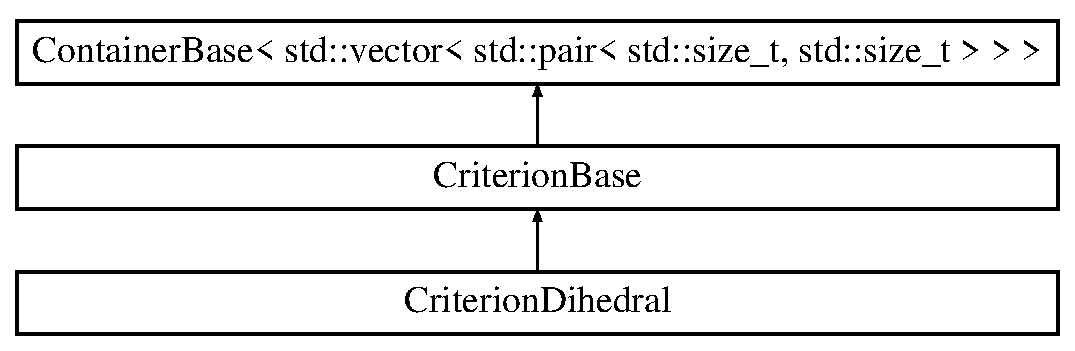
\includegraphics[height=3.000000cm]{classCriterionDihedral}
\end{center}
\end{figure}
\subsection*{Public Member Functions}
\begin{DoxyCompactItemize}
\item 
\mbox{\Hypertarget{classCriterionDihedral_a36631d04aa53d707c3f35ab1e55791d3}\label{classCriterionDihedral_a36631d04aa53d707c3f35ab1e55791d3}} 
virtual std\+::string {\bfseries get\+Type} () const override
\item 
\mbox{\Hypertarget{classCriterionDihedral_a3790c79412e3a3f3a95ae5dfd3bd070c}\label{classCriterionDihedral_a3790c79412e3a3f3a95ae5dfd3bd070c}} 
bool {\bfseries valid} (const std\+::vector$<$ \mbox{\hyperlink{classMolecule}{Molecule}} $>$ \&reactants, const R\+E\+A\+L\+V\+EC \&box\+Dimensions)
\end{DoxyCompactItemize}
\subsection*{Protected Member Functions}
\begin{DoxyCompactItemize}
\item 
\mbox{\Hypertarget{classCriterionDihedral_a3b54f8c34e03a84ae42f0623fc4ed7df}\label{classCriterionDihedral_a3b54f8c34e03a84ae42f0623fc4ed7df}} 
virtual \mbox{\hyperlink{classCriterionDihedral}{Criterion\+Dihedral}} $\ast$ {\bfseries clone\+\_\+impl} () const override
\end{DoxyCompactItemize}
\subsection*{Additional Inherited Members}


The documentation for this class was generated from the following file\+:\begin{DoxyCompactItemize}
\item 
reaction/criterion\+Derived.\+hpp\end{DoxyCompactItemize}

\hypertarget{classCriterionDistance}{}\section{Criterion\+Distance Class Reference}
\label{classCriterionDistance}\index{Criterion\+Distance@{Criterion\+Distance}}
Inheritance diagram for Criterion\+Distance\+:\begin{figure}[H]
\begin{center}
\leavevmode
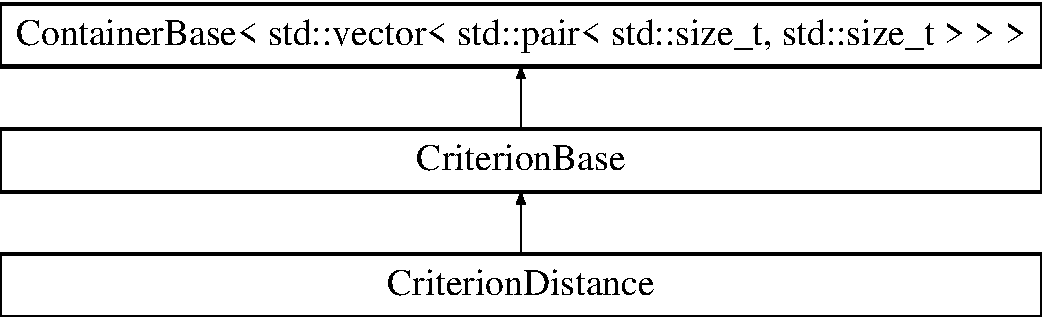
\includegraphics[height=3.000000cm]{classCriterionDistance}
\end{center}
\end{figure}
\subsection*{Public Member Functions}
\begin{DoxyCompactItemize}
\item 
\mbox{\Hypertarget{classCriterionDistance_a686f1f8b494a7ec3df4ee8dae3893a6b}\label{classCriterionDistance_a686f1f8b494a7ec3df4ee8dae3893a6b}} 
virtual std\+::string {\bfseries get\+Type} () const override
\item 
\mbox{\Hypertarget{classCriterionDistance_a8ac92b3bb74ea80a80b78aa1566e46c7}\label{classCriterionDistance_a8ac92b3bb74ea80a80b78aa1566e46c7}} 
bool {\bfseries valid} (const std\+::vector$<$ \mbox{\hyperlink{classMolecule}{Molecule}} $>$ \&reactants, const R\+E\+A\+L\+V\+EC \&box\+Dimensions)
\end{DoxyCompactItemize}
\subsection*{Protected Member Functions}
\begin{DoxyCompactItemize}
\item 
\mbox{\Hypertarget{classCriterionDistance_a5445eb7e4b31b679594aca24fcdbf06a}\label{classCriterionDistance_a5445eb7e4b31b679594aca24fcdbf06a}} 
virtual \mbox{\hyperlink{classCriterionDistance}{Criterion\+Distance}} $\ast$ {\bfseries clone\+\_\+impl} () const override
\end{DoxyCompactItemize}
\subsection*{Additional Inherited Members}


The documentation for this class was generated from the following file\+:\begin{DoxyCompactItemize}
\item 
reaction/criterion\+Derived.\+hpp\end{DoxyCompactItemize}

\hypertarget{classEnergyParserBase}{}\section{Energy\+Parser\+Base Class Reference}
\label{classEnergyParserBase}\index{Energy\+Parser\+Base@{Energy\+Parser\+Base}}
Inheritance diagram for Energy\+Parser\+Base\+:\begin{figure}[H]
\begin{center}
\leavevmode
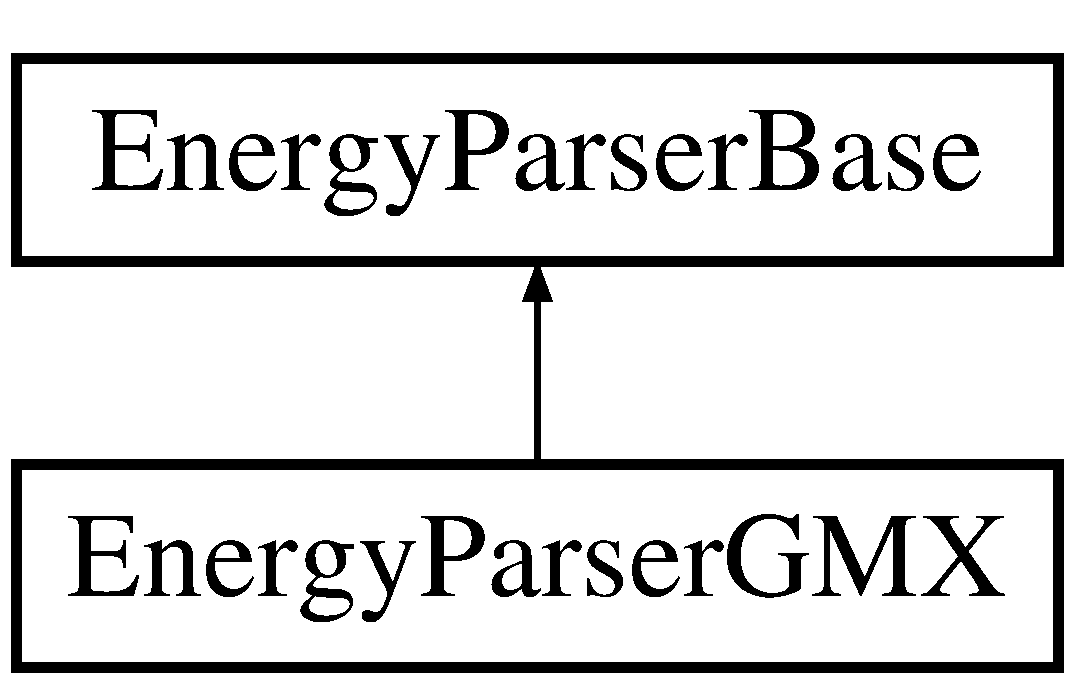
\includegraphics[height=2.000000cm]{classEnergyParserBase}
\end{center}
\end{figure}
\subsection*{Public Member Functions}
\begin{DoxyCompactItemize}
\item 
\mbox{\Hypertarget{classEnergyParserBase_aa5519bffcf0a4b98248f9a38445ab4a2}\label{classEnergyParserBase_aa5519bffcf0a4b98248f9a38445ab4a2}} 
virtual R\+E\+AL {\bfseries read\+Potential\+Energy\+Difference} (const std\+::size\+\_\+t \&, const std\+::size\+\_\+t \&)=0
\item 
\mbox{\Hypertarget{classEnergyParserBase_ae8348bff0f710ce4c1006e215eb1d307}\label{classEnergyParserBase_ae8348bff0f710ce4c1006e215eb1d307}} 
virtual void {\bfseries setup} (const \mbox{\hyperlink{classParameters}{Parameters}} \&)=0
\end{DoxyCompactItemize}


The documentation for this class was generated from the following file\+:\begin{DoxyCompactItemize}
\item 
parser/energy\+Parser\+Base.\+hpp\end{DoxyCompactItemize}

\hypertarget{classEnergyParserGMX}{}\section{Energy\+Parser\+G\+MX Class Reference}
\label{classEnergyParserGMX}\index{Energy\+Parser\+G\+MX@{Energy\+Parser\+G\+MX}}
Inheritance diagram for Energy\+Parser\+G\+MX\+:\begin{figure}[H]
\begin{center}
\leavevmode
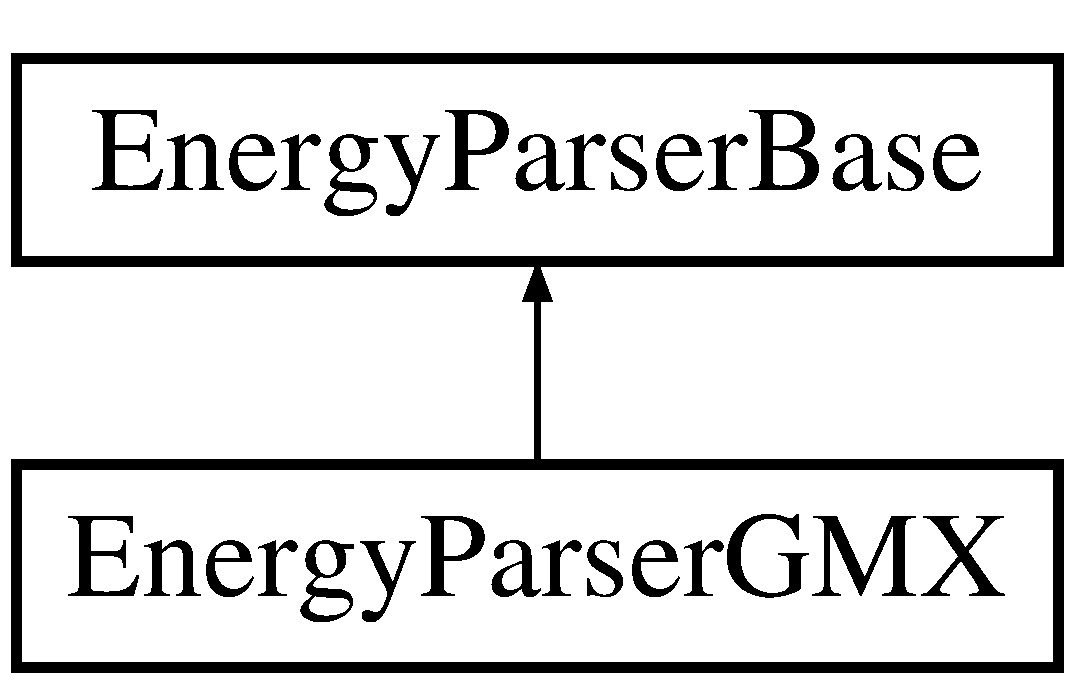
\includegraphics[height=2.000000cm]{classEnergyParserGMX}
\end{center}
\end{figure}
\subsection*{Public Member Functions}
\begin{DoxyCompactItemize}
\item 
\mbox{\Hypertarget{classEnergyParserGMX_a8dbcd08101660ce96628155c3ccc2063}\label{classEnergyParserGMX_a8dbcd08101660ce96628155c3ccc2063}} 
R\+E\+AL {\bfseries read\+Potential\+Energy\+Difference} (const std\+::size\+\_\+t \&, const std\+::size\+\_\+t \&)
\item 
\mbox{\Hypertarget{classEnergyParserGMX_ac1159165d7a5f9c5d82f46bbd1834e38}\label{classEnergyParserGMX_ac1159165d7a5f9c5d82f46bbd1834e38}} 
void {\bfseries setup} (const \mbox{\hyperlink{classParameters}{Parameters}} \&)
\end{DoxyCompactItemize}


The documentation for this class was generated from the following files\+:\begin{DoxyCompactItemize}
\item 
parser/energy\+Parser\+G\+M\+X.\+hpp\item 
parser/energy\+Parser\+G\+M\+X.\+cpp\end{DoxyCompactItemize}

\hypertarget{classEngineBase}{}\section{Engine\+Base Class Reference}
\label{classEngineBase}\index{Engine\+Base@{Engine\+Base}}
Inheritance diagram for Engine\+Base\+:\begin{figure}[H]
\begin{center}
\leavevmode
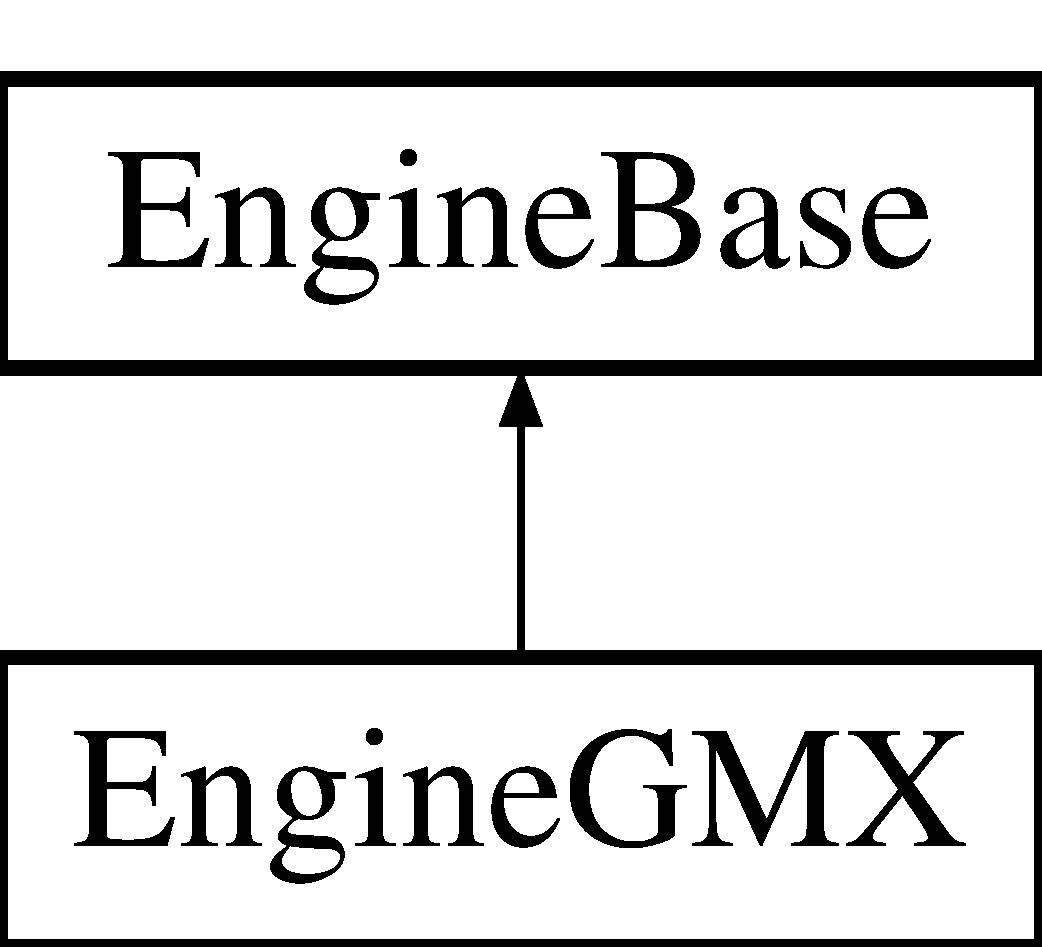
\includegraphics[height=2.000000cm]{classEngineBase}
\end{center}
\end{figure}
\subsection*{Public Member Functions}
\begin{DoxyCompactItemize}
\item 
\mbox{\Hypertarget{classEngineBase_a823f088e68a7d10c8ebe18b775629662}\label{classEngineBase_a823f088e68a7d10c8ebe18b775629662}} 
virtual void {\bfseries setup} (const \mbox{\hyperlink{classParameters}{Parameters}} \&)=0
\item 
\mbox{\Hypertarget{classEngineBase_a0ef622ef971e22057befd63b9e368c6f}\label{classEngineBase_a0ef622ef971e22057befd63b9e368c6f}} 
virtual void {\bfseries verify\+Executable} ()=0
\item 
\mbox{\Hypertarget{classEngineBase_add0a383b0c76ee4ffabf0e5941288161}\label{classEngineBase_add0a383b0c76ee4ffabf0e5941288161}} 
virtual void {\bfseries run\+MD} (const std\+::size\+\_\+t \&)=0
\item 
\mbox{\Hypertarget{classEngineBase_ad5334c6c938b757a04916a9502d9c3d6}\label{classEngineBase_ad5334c6c938b757a04916a9502d9c3d6}} 
virtual void {\bfseries run\+M\+D\+Initial} ()=0
\item 
\mbox{\Hypertarget{classEngineBase_a548dbdbed3c16043f1b188717c8c95f8}\label{classEngineBase_a548dbdbed3c16043f1b188717c8c95f8}} 
virtual void {\bfseries run\+M\+D\+Appending} (const std\+::size\+\_\+t \&, const std\+::size\+\_\+t \&)=0
\item 
\mbox{\Hypertarget{classEngineBase_a603c3fed18ba5fcb1961e0811d6643f2}\label{classEngineBase_a603c3fed18ba5fcb1961e0811d6643f2}} 
virtual bool {\bfseries run\+Relaxation} (const std\+::size\+\_\+t \&)=0
\item 
\mbox{\Hypertarget{classEngineBase_ad826ddbf873563ce03c38568e0118bcf}\label{classEngineBase_ad826ddbf873563ce03c38568e0118bcf}} 
virtual void {\bfseries run\+Energy\+Computation} (const std\+::size\+\_\+t \&, const std\+::size\+\_\+t \&)=0
\item 
\mbox{\Hypertarget{classEngineBase_a1de376fba7c90dc89e8a05e5787a442c}\label{classEngineBase_a1de376fba7c90dc89e8a05e5787a442c}} 
virtual void {\bfseries cleanup} (const std\+::size\+\_\+t \&)=0
\end{DoxyCompactItemize}
\subsection*{Protected Member Functions}
\begin{DoxyCompactItemize}
\item 
\mbox{\Hypertarget{classEngineBase_a939dfd79b49b4f3f7e41bc6b3a93c8b5}\label{classEngineBase_a939dfd79b49b4f3f7e41bc6b3a93c8b5}} 
{\footnotesize template$<$typename... Args$>$ }\\void {\bfseries execute} (const char $\ast$, Args \&\&... args)
\item 
\mbox{\Hypertarget{classEngineBase_a339cd7c8de521c66ee4ca97c641e0607}\label{classEngineBase_a339cd7c8de521c66ee4ca97c641e0607}} 
{\footnotesize template$<$typename... Args$>$ }\\void {\bfseries execute} (std\+::string \&, const char $\ast$, Args \&\&... args)
\end{DoxyCompactItemize}


The documentation for this class was generated from the following file\+:\begin{DoxyCompactItemize}
\item 
engine/engine\+Base.\+hpp\end{DoxyCompactItemize}

\hypertarget{classEngineGMX}{}\section{Engine\+G\+MX Class Reference}
\label{classEngineGMX}\index{Engine\+G\+MX@{Engine\+G\+MX}}
Inheritance diagram for Engine\+G\+MX\+:\begin{figure}[H]
\begin{center}
\leavevmode
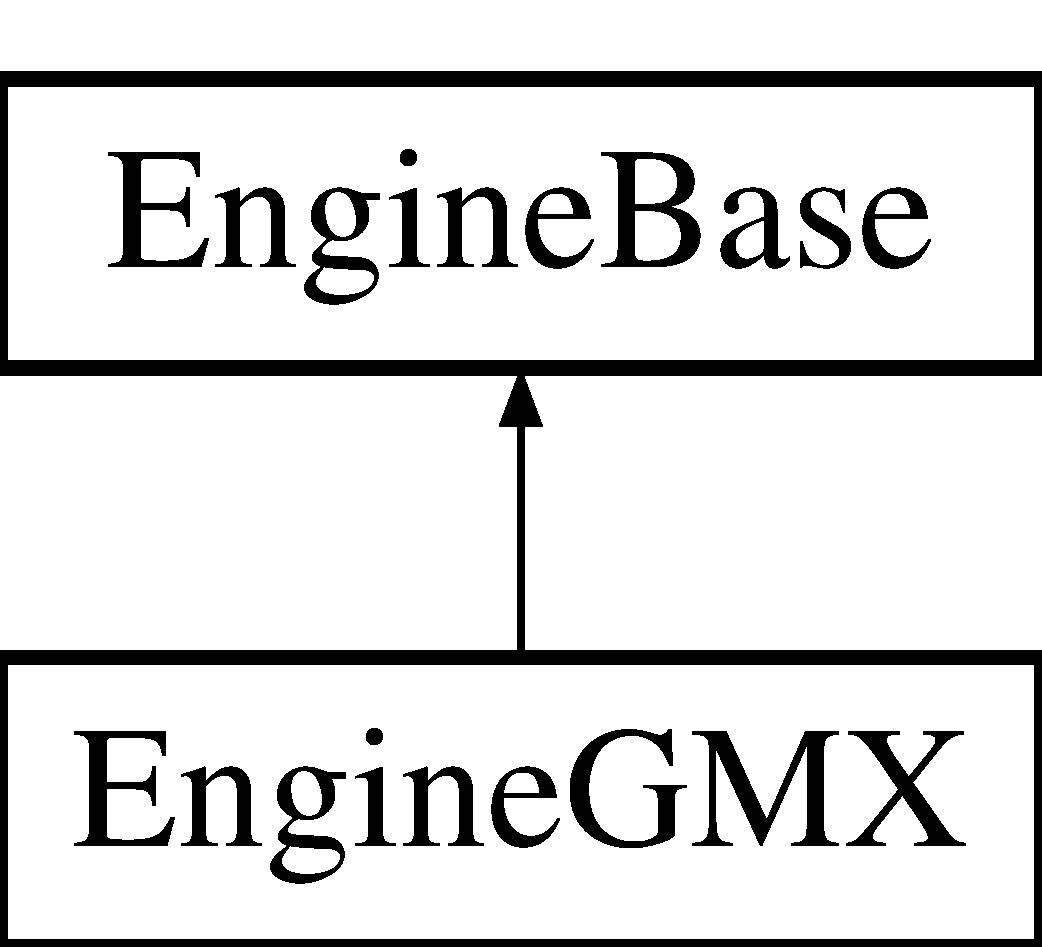
\includegraphics[height=2.000000cm]{classEngineGMX}
\end{center}
\end{figure}
\subsection*{Public Member Functions}
\begin{DoxyCompactItemize}
\item 
\mbox{\Hypertarget{classEngineGMX_ae56d6737c759974e794a3286f485c892}\label{classEngineGMX_ae56d6737c759974e794a3286f485c892}} 
void {\bfseries setup} (const \mbox{\hyperlink{classParameters}{Parameters}} \&)
\item 
\mbox{\Hypertarget{classEngineGMX_ae995206760c8c24ae1d6297644dd8525}\label{classEngineGMX_ae995206760c8c24ae1d6297644dd8525}} 
void {\bfseries verify\+Executable} ()
\item 
\mbox{\Hypertarget{classEngineGMX_a0215383c1101ce6a6f20a4bd7361b891}\label{classEngineGMX_a0215383c1101ce6a6f20a4bd7361b891}} 
void {\bfseries run\+MD} (const std\+::size\+\_\+t \&)
\item 
\mbox{\Hypertarget{classEngineGMX_a89fcede457959fc7ba656dd0fa1767ac}\label{classEngineGMX_a89fcede457959fc7ba656dd0fa1767ac}} 
void {\bfseries run\+M\+D\+Initial} ()
\item 
\mbox{\Hypertarget{classEngineGMX_a909fb34f58e0fb27d26a3434d0d15a8a}\label{classEngineGMX_a909fb34f58e0fb27d26a3434d0d15a8a}} 
void {\bfseries run\+M\+D\+Appending} (const std\+::size\+\_\+t \&, const std\+::size\+\_\+t \&)
\item 
\mbox{\Hypertarget{classEngineGMX_a3f58c6d243a78bb9381ce22169733b1c}\label{classEngineGMX_a3f58c6d243a78bb9381ce22169733b1c}} 
bool {\bfseries run\+Relaxation} (const std\+::size\+\_\+t \&)
\item 
\mbox{\Hypertarget{classEngineGMX_a692cc4814a50f113214db669529c8ad4}\label{classEngineGMX_a692cc4814a50f113214db669529c8ad4}} 
void {\bfseries run\+Energy\+Computation} (const std\+::size\+\_\+t \&, const std\+::size\+\_\+t \&)
\item 
\mbox{\Hypertarget{classEngineGMX_aeaabdd6cdaeda2f51f366b4a2788051b}\label{classEngineGMX_aeaabdd6cdaeda2f51f366b4a2788051b}} 
void {\bfseries cleanup} (const std\+::size\+\_\+t \&)
\end{DoxyCompactItemize}
\subsection*{Additional Inherited Members}


The documentation for this class was generated from the following files\+:\begin{DoxyCompactItemize}
\item 
engine/engine\+G\+M\+X.\+hpp\item 
engine/engine\+G\+M\+X.\+cpp\end{DoxyCompactItemize}

\hypertarget{classMolecule}{}\section{Molecule Class Reference}
\label{classMolecule}\index{Molecule@{Molecule}}
Inheritance diagram for Molecule\+:\begin{figure}[H]
\begin{center}
\leavevmode
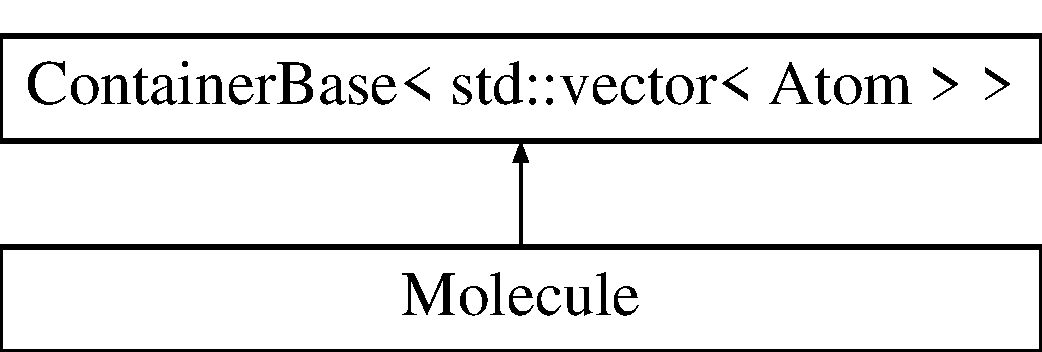
\includegraphics[height=2.000000cm]{classMolecule}
\end{center}
\end{figure}
\subsection*{Public Member Functions}
\begin{DoxyCompactItemize}
\item 
\mbox{\Hypertarget{classMolecule_a4940ffb3d3e6c935e3fc2bccbf7107d3}\label{classMolecule_a4940ffb3d3e6c935e3fc2bccbf7107d3}} 
void {\bfseries set\+ID} (std\+::size\+\_\+t id)
\item 
\mbox{\Hypertarget{classMolecule_a77d5303c4ff048502b73adba7207ed79}\label{classMolecule_a77d5303c4ff048502b73adba7207ed79}} 
void {\bfseries set\+Name} (std\+::string name)
\item 
\mbox{\Hypertarget{classMolecule_af4313873dda8ed9eee321c43fee310a6}\label{classMolecule_af4313873dda8ed9eee321c43fee310a6}} 
const auto \& {\bfseries get\+ID} () const
\item 
\mbox{\Hypertarget{classMolecule_abb3cefe3898d802d6684ad47993dd159}\label{classMolecule_abb3cefe3898d802d6684ad47993dd159}} 
const auto \& {\bfseries get\+Name} () const
\item 
\mbox{\Hypertarget{classMolecule_a2fe20ffab84ba21ddf9c7f489a52b4e6}\label{classMolecule_a2fe20ffab84ba21ddf9c7f489a52b4e6}} 
auto {\bfseries add\+Atom} (\mbox{\hyperlink{structAtom}{Atom}} a)
\item 
\mbox{\Hypertarget{classMolecule_a5961760d11096237c00c6463097c357d}\label{classMolecule_a5961760d11096237c00c6463097c357d}} 
auto {\bfseries add\+Atom} (std\+::size\+\_\+t id, std\+::string name)
\item 
\mbox{\Hypertarget{classMolecule_a3e6f6cc7048d35137a581d7fe703d040}\label{classMolecule_a3e6f6cc7048d35137a581d7fe703d040}} 
const \mbox{\hyperlink{structAtom}{Atom}} \& {\bfseries get\+Atom} (std\+::size\+\_\+t id) const
\item 
\mbox{\Hypertarget{classMolecule_a1570c9668e3c060090831a64bc516f1d}\label{classMolecule_a1570c9668e3c060090831a64bc516f1d}} 
void {\bfseries remove\+Atom} (\mbox{\hyperlink{structAtom}{Atom}} \&element)
\item 
\mbox{\Hypertarget{classMolecule_a5825adf80b9339a13fec9c61bcc37c8f}\label{classMolecule_a5825adf80b9339a13fec9c61bcc37c8f}} 
void {\bfseries remove\+Atom} (std\+::size\+\_\+t id)
\item 
\mbox{\Hypertarget{classMolecule_a3d5c5e4e5e5661c6ae101e8677daf5a2}\label{classMolecule_a3d5c5e4e5e5661c6ae101e8677daf5a2}} 
bool {\bfseries contains\+Atom} (\mbox{\hyperlink{structAtom}{Atom}} \&element) const
\item 
\mbox{\Hypertarget{classMolecule_a6f27921b5f6c57099a5012ceb4c59ba5}\label{classMolecule_a6f27921b5f6c57099a5012ceb4c59ba5}} 
bool {\bfseries contains\+Atom} (std\+::size\+\_\+t id) const
\item 
\mbox{\Hypertarget{classMolecule_a874d801249ed4ecc7546f966569fb46e}\label{classMolecule_a874d801249ed4ecc7546f966569fb46e}} 
bool {\bfseries contains\+Atom} (std\+::string name) const
\item 
\mbox{\Hypertarget{classMolecule_a3ac4752cf4109ce203ce2915ca78070c}\label{classMolecule_a3ac4752cf4109ce203ce2915ca78070c}} 
bool {\bfseries empty} () const
\item 
\mbox{\Hypertarget{classMolecule_afe579bbd0c5fbbc3c13e47dfbcc6365a}\label{classMolecule_afe579bbd0c5fbbc3c13e47dfbcc6365a}} 
bool {\bfseries operator==} (const \mbox{\hyperlink{classMolecule}{Molecule}} \&other) const
\item 
\mbox{\Hypertarget{classMolecule_ad45ebe1227fb20d3b67b6eba04ff8e06}\label{classMolecule_ad45ebe1227fb20d3b67b6eba04ff8e06}} 
bool {\bfseries operator!=} (const \mbox{\hyperlink{classMolecule}{Molecule}} \&other) const
\item 
\mbox{\Hypertarget{classMolecule_a46103a552f2114e0f37b3ec325249da7}\label{classMolecule_a46103a552f2114e0f37b3ec325249da7}} 
bool {\bfseries operator$<$} (const \mbox{\hyperlink{classMolecule}{Molecule}} \&other) const
\item 
\mbox{\Hypertarget{classMolecule_a428eb340f80dcae8d48ea26a3204b311}\label{classMolecule_a428eb340f80dcae8d48ea26a3204b311}} 
bool {\bfseries operator$>$} (const \mbox{\hyperlink{classMolecule}{Molecule}} \&other) const
\end{DoxyCompactItemize}
\subsection*{Friends}
\begin{DoxyCompactItemize}
\item 
\mbox{\Hypertarget{classMolecule_a0b4533cd3ad55d6afaba9d291ded714b}\label{classMolecule_a0b4533cd3ad55d6afaba9d291ded714b}} 
std\+::ostream \& {\bfseries operator$<$$<$} (std\+::ostream \&, const \mbox{\hyperlink{structAtom}{Atom}} \&)
\end{DoxyCompactItemize}
\subsection*{Additional Inherited Members}


The documentation for this class was generated from the following files\+:\begin{DoxyCompactItemize}
\item 
container/molecule.\+hpp\item 
container/molecule.\+cpp\end{DoxyCompactItemize}

\hypertarget{classParameters}{}\section{Parameters Class Reference}
\label{classParameters}\index{Parameters@{Parameters}}
\subsection*{Public Member Functions}
\begin{DoxyCompactItemize}
\item 
\mbox{\Hypertarget{classParameters_a9c0282e8d18dc439e76285fa8201d9fa}\label{classParameters_a9c0282e8d18dc439e76285fa8201d9fa}} 
{\bfseries Parameters} (int, char $\ast$\mbox{[}$\,$\mbox{]})
\item 
\mbox{\Hypertarget{classParameters_af21c1953c78336642586e55f6f2fb1c6}\label{classParameters_af21c1953c78336642586e55f6f2fb1c6}} 
const auto \& {\bfseries get\+Option} (const std\+::string \&s) const
\item 
\mbox{\Hypertarget{classParameters_ad60464f44cc2e44ca371c1bdddac7ee2}\label{classParameters_ad60464f44cc2e44ca371c1bdddac7ee2}} 
const auto \& {\bfseries get\+Engine\+Type} () const
\item 
\mbox{\Hypertarget{classParameters_a251e6cc559a6bc520ecc49d6eae0e83c}\label{classParameters_a251e6cc559a6bc520ecc49d6eae0e83c}} 
const auto \& {\bfseries get\+Simulation\+Mode} () const
\item 
\mbox{\Hypertarget{classParameters_ab7aa696880b7d6952faa1756ff378988}\label{classParameters_ab7aa696880b7d6952faa1756ff378988}} 
const auto \& {\bfseries get\+Simulation\+Algorithm} () const
\item 
\mbox{\Hypertarget{classParameters_a096a247b3587ee5a98f5f7abe967e537}\label{classParameters_a096a247b3587ee5a98f5f7abe967e537}} 
std\+::string {\bfseries str} () const
\item 
\mbox{\Hypertarget{classParameters_ad1e257b92912d96e82eb912a8d952dec}\label{classParameters_ad1e257b92912d96e82eb912a8d952dec}} 
{\footnotesize template$<$$>$ }\\std\+::string {\bfseries formatted} (const std\+::string \&name, const std\+::vector$<$ std\+::string $>$ \&values) const
\end{DoxyCompactItemize}


The documentation for this class was generated from the following files\+:\begin{DoxyCompactItemize}
\item 
parameters/parameters.\+hpp\item 
parameters/parameters.\+cpp\end{DoxyCompactItemize}

\hypertarget{classReactionBase}{}\section{Reaction\+Base Class Reference}
\label{classReactionBase}\index{Reaction\+Base@{Reaction\+Base}}
Inheritance diagram for Reaction\+Base\+:\begin{figure}[H]
\begin{center}
\leavevmode
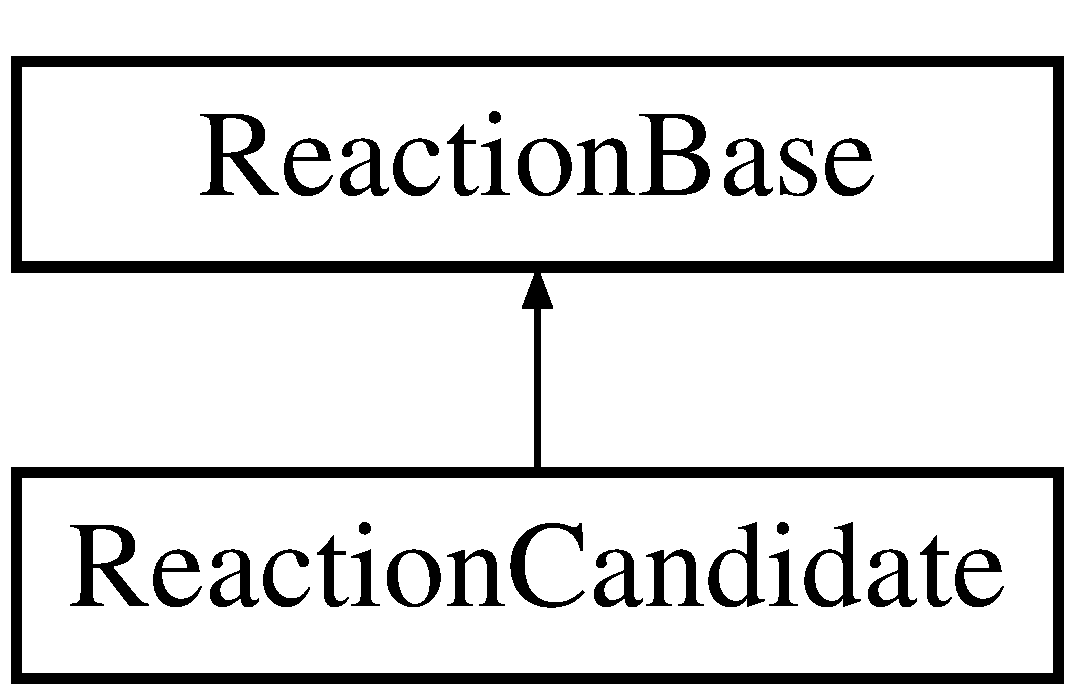
\includegraphics[height=2.000000cm]{classReactionBase}
\end{center}
\end{figure}
\subsection*{Public Member Functions}
\begin{DoxyCompactItemize}
\item 
\mbox{\Hypertarget{classReactionBase_a31c1e3e98e4735e62a1b59fb50d58189}\label{classReactionBase_a31c1e3e98e4735e62a1b59fb50d58189}} 
{\bfseries Reaction\+Base} (const \mbox{\hyperlink{classReactionBase}{Reaction\+Base}} \&)
\item 
\mbox{\Hypertarget{classReactionBase_a68cbcd543251905a1cacd65222e758b6}\label{classReactionBase_a68cbcd543251905a1cacd65222e758b6}} 
{\bfseries Reaction\+Base} (\mbox{\hyperlink{classReactionBase}{Reaction\+Base}} \&\&)=default
\item 
\mbox{\Hypertarget{classReactionBase_a8c9f416cebd93e12b25d25f23369bc4d}\label{classReactionBase_a8c9f416cebd93e12b25d25f23369bc4d}} 
\mbox{\hyperlink{classReactionBase}{Reaction\+Base}} \& {\bfseries operator=} (const \mbox{\hyperlink{classReactionBase}{Reaction\+Base}} \&)=delete
\item 
\mbox{\Hypertarget{classReactionBase_ac82aa6be6c875ef2e0814bc80b37e89e}\label{classReactionBase_ac82aa6be6c875ef2e0814bc80b37e89e}} 
\mbox{\hyperlink{classReactionBase}{Reaction\+Base}} \& {\bfseries operator=} (\mbox{\hyperlink{classReactionBase}{Reaction\+Base}} \&\&)=default
\item 
\mbox{\Hypertarget{classReactionBase_ac8a3d47ec48f88eb9cabdb419d494840}\label{classReactionBase_ac8a3d47ec48f88eb9cabdb419d494840}} 
void {\bfseries set\+Name} (const std\+::string \&n)
\item 
\mbox{\Hypertarget{classReactionBase_ae14a20704f5ffa9f97b0e218267fcfde}\label{classReactionBase_ae14a20704f5ffa9f97b0e218267fcfde}} 
const auto \& {\bfseries get\+Name} () const
\item 
\mbox{\Hypertarget{classReactionBase_abb467dc64b5eae8719fb32197f33ccda}\label{classReactionBase_abb467dc64b5eae8719fb32197f33ccda}} 
void {\bfseries set\+Reaction\+Energy} (const R\+E\+AL \&e)
\item 
\mbox{\Hypertarget{classReactionBase_a36387f94f86afc9aa09e0803b1bdff77}\label{classReactionBase_a36387f94f86afc9aa09e0803b1bdff77}} 
const auto \& {\bfseries get\+Reaction\+Energy} () const
\item 
\mbox{\Hypertarget{classReactionBase_a320d3cc723874f2274cda66f1d06aea0}\label{classReactionBase_a320d3cc723874f2274cda66f1d06aea0}} 
void {\bfseries set\+Activation\+Energy} (const R\+E\+AL \&e)
\item 
\mbox{\Hypertarget{classReactionBase_a6d4674768a54a2c0e14fbe1728d000e8}\label{classReactionBase_a6d4674768a54a2c0e14fbe1728d000e8}} 
const auto \& {\bfseries get\+Activation\+Energy} () const
\item 
\mbox{\Hypertarget{classReactionBase_aef07f8ea4b7b1e2a5c845b975a483068}\label{classReactionBase_aef07f8ea4b7b1e2a5c845b975a483068}} 
void {\bfseries set\+Rate} (const std\+::vector$<$ std\+::pair$<$ R\+E\+AL, R\+E\+AL $>$$>$ r)
\item 
\mbox{\Hypertarget{classReactionBase_add55a600cdce958694340acf21d53f7c}\label{classReactionBase_add55a600cdce958694340acf21d53f7c}} 
const auto \& {\bfseries get\+Rate} () const
\item 
\mbox{\Hypertarget{classReactionBase_a95c27a29dc68337fd5952c7041e841ae}\label{classReactionBase_a95c27a29dc68337fd5952c7041e841ae}} 
const auto {\bfseries get\+Reactant} (const std\+::size\+\_\+t \&) const
\item 
\mbox{\Hypertarget{classReactionBase_acd2fb67953b08595d2b1a47178fccf17}\label{classReactionBase_acd2fb67953b08595d2b1a47178fccf17}} 
const auto \& {\bfseries get\+Reactants} () const
\item 
\mbox{\Hypertarget{classReactionBase_ac3f3c586862e81cede4de3cf578f66ba}\label{classReactionBase_ac3f3c586862e81cede4de3cf578f66ba}} 
auto \& {\bfseries get\+Reactants} ()
\item 
\mbox{\Hypertarget{classReactionBase_a14a6362a090dbe19863c96168c5d54d6}\label{classReactionBase_a14a6362a090dbe19863c96168c5d54d6}} 
const auto {\bfseries get\+Product} (const std\+::size\+\_\+t \&) const
\item 
\mbox{\Hypertarget{classReactionBase_adfa2078cd128b851e7c01857f5c201ea}\label{classReactionBase_adfa2078cd128b851e7c01857f5c201ea}} 
const auto \& {\bfseries get\+Products} () const
\item 
\mbox{\Hypertarget{classReactionBase_a401b658122ff826b798815dec0ee72d4}\label{classReactionBase_a401b658122ff826b798815dec0ee72d4}} 
auto \& {\bfseries get\+Products} ()
\item 
\mbox{\Hypertarget{classReactionBase_a90290e7188cafcc8004530ca121c4eff}\label{classReactionBase_a90290e7188cafcc8004530ca121c4eff}} 
\mbox{\hyperlink{classMolecule}{Molecule}} \& {\bfseries get\+Add\+Reactant} (const std\+::size\+\_\+t \&)
\item 
\mbox{\Hypertarget{classReactionBase_a54a123c645a586ffee09202f0d8bae87}\label{classReactionBase_a54a123c645a586ffee09202f0d8bae87}} 
\mbox{\hyperlink{classMolecule}{Molecule}} \& {\bfseries get\+Add\+Product} (const std\+::size\+\_\+t \&)
\item 
\mbox{\Hypertarget{classReactionBase_ae52ff33bd1e3712cdc1c791a656344ed}\label{classReactionBase_ae52ff33bd1e3712cdc1c791a656344ed}} 
void {\bfseries add\+Transition} (const std\+::size\+\_\+t \&, const std\+::size\+\_\+t \&, const std\+::size\+\_\+t \&, const std\+::size\+\_\+t \&)
\item 
\mbox{\Hypertarget{classReactionBase_ae98edd1217ea53a633d310977058e63a}\label{classReactionBase_ae98edd1217ea53a633d310977058e63a}} 
void {\bfseries add\+Criterion} (const std\+::vector$<$ std\+::pair$<$ std\+::size\+\_\+t, std\+::size\+\_\+t $>$$>$ \&, const std\+::pair$<$ R\+E\+AL, R\+E\+AL $>$ \&)
\item 
\mbox{\Hypertarget{classReactionBase_a35d5ce146a466fff7068efabda7f4b85}\label{classReactionBase_a35d5ce146a466fff7068efabda7f4b85}} 
void {\bfseries add\+Translation} (const std\+::vector$<$ std\+::pair$<$ std\+::size\+\_\+t, std\+::size\+\_\+t $>$$>$ \&, const R\+E\+AL \&)
\item 
\mbox{\Hypertarget{classReactionBase_a97faebca27e11db7f328d649fe2f4dc2}\label{classReactionBase_a97faebca27e11db7f328d649fe2f4dc2}} 
void {\bfseries consistency\+Check} () const
\end{DoxyCompactItemize}
\subsection*{Protected Member Functions}
\begin{DoxyCompactItemize}
\item 
\mbox{\Hypertarget{classReactionBase_a5789e10d9f987be82a84e6944aa254f9}\label{classReactionBase_a5789e10d9f987be82a84e6944aa254f9}} 
virtual std\+::string {\bfseries str} () const
\end{DoxyCompactItemize}
\subsection*{Protected Attributes}
\begin{DoxyCompactItemize}
\item 
\mbox{\Hypertarget{classReactionBase_a004e93dc692a166c7d9a7fc0fb2c7138}\label{classReactionBase_a004e93dc692a166c7d9a7fc0fb2c7138}} 
std\+::string {\bfseries name} \{\}
\item 
\mbox{\Hypertarget{classReactionBase_a550c52da47b04316b58bb0892df7c711}\label{classReactionBase_a550c52da47b04316b58bb0892df7c711}} 
std\+::vector$<$ \mbox{\hyperlink{classMolecule}{Molecule}} $>$ {\bfseries reactants} \{\}
\item 
\mbox{\Hypertarget{classReactionBase_acd868f79a10adb1b0289fe5bfef6eba9}\label{classReactionBase_acd868f79a10adb1b0289fe5bfef6eba9}} 
std\+::vector$<$ \mbox{\hyperlink{classMolecule}{Molecule}} $>$ {\bfseries products} \{\}
\item 
\mbox{\Hypertarget{classReactionBase_a6582ae367365272050cc1cd49b8be80d}\label{classReactionBase_a6582ae367365272050cc1cd49b8be80d}} 
std\+::vector$<$ \mbox{\hyperlink{structTransitionTable}{Transition\+Table}} $>$ {\bfseries transition\+Tables} \{\}
\item 
\mbox{\Hypertarget{classReactionBase_aad65650f91ccf99bfb28707144ac1c38}\label{classReactionBase_aad65650f91ccf99bfb28707144ac1c38}} 
std\+::vector$<$ \mbox{\hyperlink{structTranslationTable}{Translation\+Table}} $>$ {\bfseries translation\+Tables} \{\}
\item 
\mbox{\Hypertarget{classReactionBase_ace96bb2e98f3d9ac620466122869086c}\label{classReactionBase_ace96bb2e98f3d9ac620466122869086c}} 
R\+E\+AL {\bfseries reaction\+Energy} \{0\}
\item 
\mbox{\Hypertarget{classReactionBase_a7d16d82ee2e553e6e71d4243c930f3ef}\label{classReactionBase_a7d16d82ee2e553e6e71d4243c930f3ef}} 
R\+E\+AL {\bfseries activation\+Energy} \{0\}
\item 
\mbox{\Hypertarget{classReactionBase_a43a1cf0faf80b3508bcb9c6ec8e7a3cd}\label{classReactionBase_a43a1cf0faf80b3508bcb9c6ec8e7a3cd}} 
std\+::vector$<$ std\+::pair$<$ R\+E\+AL, R\+E\+AL $>$ $>$ {\bfseries reaction\+Rate} \{\}
\item 
\mbox{\Hypertarget{classReactionBase_ac59e985477e007151293aa34a9eeb2d4}\label{classReactionBase_ac59e985477e007151293aa34a9eeb2d4}} 
std\+::vector$<$ std\+::unique\+\_\+ptr$<$ \mbox{\hyperlink{classCriterionBase}{Criterion\+Base}} $>$ $>$ {\bfseries criterions} \{\}
\end{DoxyCompactItemize}
\subsection*{Friends}
\begin{DoxyCompactItemize}
\item 
\mbox{\Hypertarget{classReactionBase_a5ae4f004821b73cb5bd00c9bd7c0c910}\label{classReactionBase_a5ae4f004821b73cb5bd00c9bd7c0c910}} 
std\+::ostream \& {\bfseries operator$<$$<$} (std\+::ostream \&stream, const \mbox{\hyperlink{classReactionBase}{Reaction\+Base}} \&reaction)
\end{DoxyCompactItemize}


The documentation for this class was generated from the following files\+:\begin{DoxyCompactItemize}
\item 
reaction/reaction\+Base.\+hpp\item 
reaction/reaction\+Base.\+cpp\end{DoxyCompactItemize}

\hypertarget{classReactionCandidate}{}\section{Reaction\+Candidate Class Reference}
\label{classReactionCandidate}\index{Reaction\+Candidate@{Reaction\+Candidate}}
Inheritance diagram for Reaction\+Candidate\+:\begin{figure}[H]
\begin{center}
\leavevmode
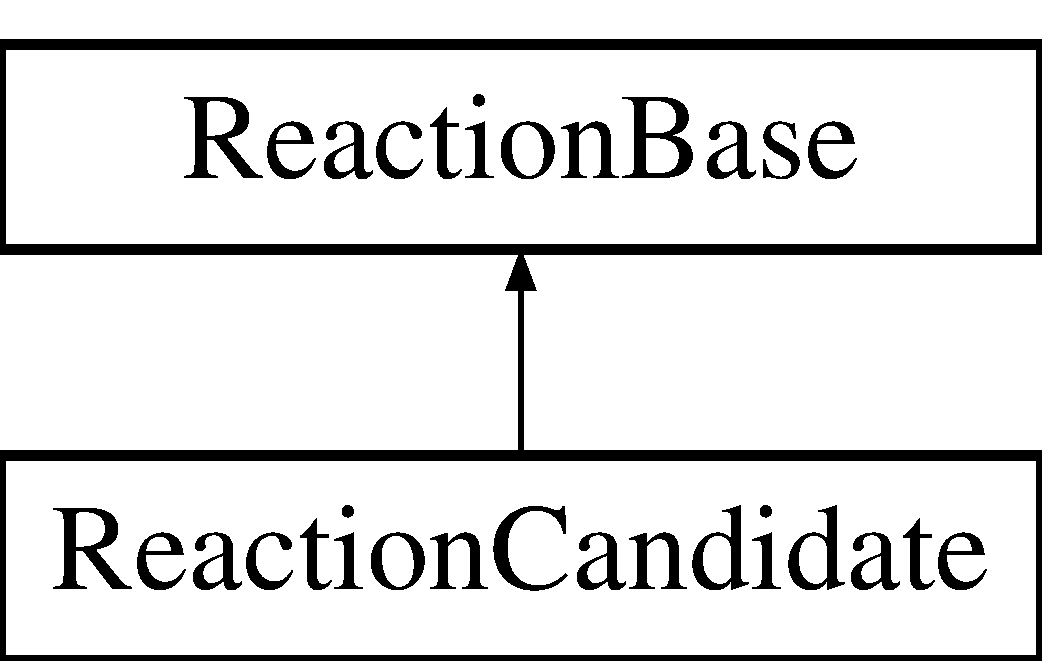
\includegraphics[height=2.000000cm]{classReactionCandidate}
\end{center}
\end{figure}
\subsection*{Public Member Functions}
\begin{DoxyCompactItemize}
\item 
\mbox{\Hypertarget{classReactionCandidate_a354fb7dab7c9d6f8587a461af02a7cab}\label{classReactionCandidate_a354fb7dab7c9d6f8587a461af02a7cab}} 
{\bfseries Reaction\+Candidate} (const \mbox{\hyperlink{classReactionBase}{Reaction\+Base}} \&)
\item 
\mbox{\Hypertarget{classReactionCandidate_ab8ef2e26cd357558bc3f1da8678fa287}\label{classReactionCandidate_ab8ef2e26cd357558bc3f1da8678fa287}} 
{\bfseries Reaction\+Candidate} (const \mbox{\hyperlink{classReactionCandidate}{Reaction\+Candidate}} \&)=default
\item 
\mbox{\Hypertarget{classReactionCandidate_aa09fe4ee2be07ed048558923200d0d6b}\label{classReactionCandidate_aa09fe4ee2be07ed048558923200d0d6b}} 
\mbox{\hyperlink{classReactionCandidate}{Reaction\+Candidate}} \& {\bfseries operator=} (const \mbox{\hyperlink{classReactionCandidate}{Reaction\+Candidate}} \&)=delete
\item 
\mbox{\Hypertarget{classReactionCandidate_aaa9808f8a1e2317a8ecafdba3595754c}\label{classReactionCandidate_aaa9808f8a1e2317a8ecafdba3595754c}} 
{\bfseries Reaction\+Candidate} (\mbox{\hyperlink{classReactionCandidate}{Reaction\+Candidate}} \&\&)=default
\item 
\mbox{\Hypertarget{classReactionCandidate_afc2a6b341b33532357d3fe6cf377b603}\label{classReactionCandidate_afc2a6b341b33532357d3fe6cf377b603}} 
\mbox{\hyperlink{classReactionCandidate}{Reaction\+Candidate}} \& {\bfseries operator=} (\mbox{\hyperlink{classReactionCandidate}{Reaction\+Candidate}} \&\&)=default
\item 
\mbox{\Hypertarget{classReactionCandidate_a62a059b5040f22b857dfeb267bb91d6a}\label{classReactionCandidate_a62a059b5040f22b857dfeb267bb91d6a}} 
R\+E\+AL {\bfseries get\+Current\+Reaction\+Rate\+Value} () const
\item 
\mbox{\Hypertarget{classReactionCandidate_a6b563ebd5094f392d1f777673c004a63}\label{classReactionCandidate_a6b563ebd5094f392d1f777673c004a63}} 
R\+E\+AL {\bfseries get\+Current\+Distance\+Value} () const
\item 
\mbox{\Hypertarget{classReactionCandidate_a42331f76746fbad22cd1059078d8214d}\label{classReactionCandidate_a42331f76746fbad22cd1059078d8214d}} 
void {\bfseries update\+Reactant} (const std\+::size\+\_\+t, const \mbox{\hyperlink{classMolecule}{Molecule}} \&)
\item 
\mbox{\Hypertarget{classReactionCandidate_ac6125505b071fa735518bb7b9b7c0a6e}\label{classReactionCandidate_ac6125505b071fa735518bb7b9b7c0a6e}} 
void {\bfseries apply\+Transitions} ()
\item 
\mbox{\Hypertarget{classReactionCandidate_a224f6dbafedbbb66e6b58389db328287}\label{classReactionCandidate_a224f6dbafedbbb66e6b58389db328287}} 
void {\bfseries apply\+Translations} ()
\item 
\mbox{\Hypertarget{classReactionCandidate_a80c2effc2e708c0474135808b34c209c}\label{classReactionCandidate_a80c2effc2e708c0474135808b34c209c}} 
bool {\bfseries valid} (const R\+E\+A\+L\+V\+EC \&)
\item 
\mbox{\Hypertarget{classReactionCandidate_aef127b6ebd265c29d26c285bebb5dc57}\label{classReactionCandidate_aef127b6ebd265c29d26c285bebb5dc57}} 
std\+::string {\bfseries short\+Info} () const
\end{DoxyCompactItemize}
\subsection*{Additional Inherited Members}


The documentation for this class was generated from the following files\+:\begin{DoxyCompactItemize}
\item 
reaction/reaction\+Candidate.\+hpp\item 
reaction/reaction\+Candidate.\+cpp\end{DoxyCompactItemize}

\hypertarget{classReactionParser}{}\section{Reaction\+Parser Class Reference}
\label{classReactionParser}\index{Reaction\+Parser@{Reaction\+Parser}}
\subsection*{Public Member Functions}
\begin{DoxyCompactItemize}
\item 
\mbox{\Hypertarget{classReactionParser_aed8877fa71830d708ac5094e2e48a0f2}\label{classReactionParser_aed8877fa71830d708ac5094e2e48a0f2}} 
\mbox{\hyperlink{classReactionBase}{Reaction\+Base}} {\bfseries read} (const std\+::string \&)
\item 
\mbox{\Hypertarget{classReactionParser_af9e8eb32819c7a054be382f8df4e1cc1}\label{classReactionParser_af9e8eb32819c7a054be382f8df4e1cc1}} 
std\+::string {\bfseries write\+Example} ()
\end{DoxyCompactItemize}


The documentation for this class was generated from the following files\+:\begin{DoxyCompactItemize}
\item 
parser/reaction\+Parser.\+hpp\item 
parser/reaction\+Parser.\+cpp\end{DoxyCompactItemize}

\hypertarget{classSimulatorBase}{}\section{Simulator\+Base Class Reference}
\label{classSimulatorBase}\index{Simulator\+Base@{Simulator\+Base}}
Inheritance diagram for Simulator\+Base\+:\begin{figure}[H]
\begin{center}
\leavevmode
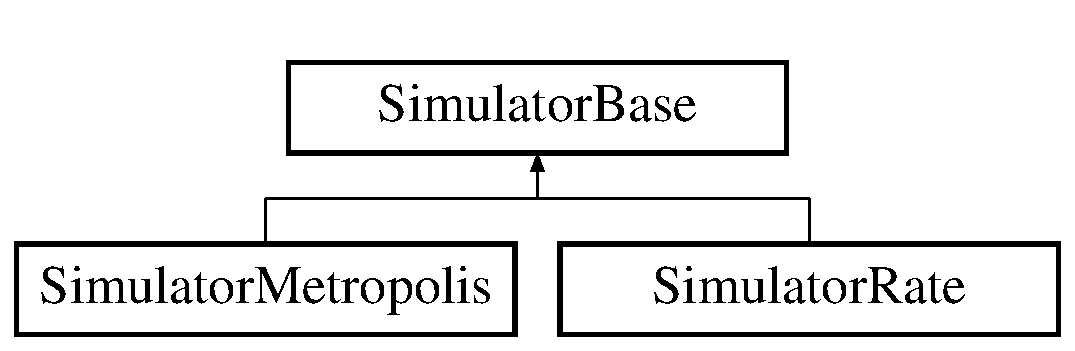
\includegraphics[height=2.000000cm]{classSimulatorBase}
\end{center}
\end{figure}
\subsection*{Public Member Functions}
\begin{DoxyCompactItemize}
\item 
\mbox{\Hypertarget{classSimulatorBase_a5f4de392eb878221ee6659e0ba74f872}\label{classSimulatorBase_a5f4de392eb878221ee6659e0ba74f872}} 
void {\bfseries run} ()
\item 
\mbox{\Hypertarget{classSimulatorBase_abf93602f7d449518be2bdbe1587a660e}\label{classSimulatorBase_abf93602f7d449518be2bdbe1587a660e}} 
void {\bfseries write\+Restart\+File} (const \mbox{\hyperlink{classParameters}{Parameters}} \&) const
\item 
\mbox{\Hypertarget{classSimulatorBase_ab62968759e46cac079187d96b4e581a1}\label{classSimulatorBase_ab62968759e46cac079187d96b4e581a1}} 
virtual void {\bfseries setup} (const \mbox{\hyperlink{classParameters}{Parameters}} \&)
\item 
\mbox{\Hypertarget{classSimulatorBase_a0fec722db46abb94bbf9446fd4064f89}\label{classSimulatorBase_a0fec722db46abb94bbf9446fd4064f89}} 
virtual void {\bfseries finish} ()=0
\item 
\mbox{\Hypertarget{classSimulatorBase_a7d89155f2b293deebd6eaf79ba1bb76d}\label{classSimulatorBase_a7d89155f2b293deebd6eaf79ba1bb76d}} 
auto {\bfseries get\+N\+Cycles} () const
\end{DoxyCompactItemize}
\subsection*{Protected Member Functions}
\begin{DoxyCompactItemize}
\item 
\mbox{\Hypertarget{classSimulatorBase_a92300915ac3d7c0812f5390068a2c23d}\label{classSimulatorBase_a92300915ac3d7c0812f5390068a2c23d}} 
void {\bfseries md\+Sequence} ()
\item 
\mbox{\Hypertarget{classSimulatorBase_af463a10b1c1c8c2df0b46e87f3d3dfac}\label{classSimulatorBase_af463a10b1c1c8c2df0b46e87f3d3dfac}} 
virtual void {\bfseries reactive\+Step} ()=0
\item 
\mbox{\Hypertarget{classSimulatorBase_a0fcd514966117c48c810137e0177009c}\label{classSimulatorBase_a0fcd514966117c48c810137e0177009c}} 
virtual bool {\bfseries acceptance} (const \mbox{\hyperlink{classReactionCandidate}{Reaction\+Candidate}} \&)=0
\end{DoxyCompactItemize}
\subsection*{Protected Attributes}
\begin{DoxyCompactItemize}
\item 
\mbox{\Hypertarget{classSimulatorBase_a5265c38f77e3fe7f04f02ec446c5220c}\label{classSimulatorBase_a5265c38f77e3fe7f04f02ec446c5220c}} 
\mbox{\hyperlink{classUniverse}{Universe}} {\bfseries universe} \{\}
\item 
\mbox{\Hypertarget{classSimulatorBase_ae53ac9ac72ac434790a8a19bd1828736}\label{classSimulatorBase_ae53ac9ac72ac434790a8a19bd1828736}} 
std\+::unique\+\_\+ptr$<$ \mbox{\hyperlink{classEngineBase}{Engine\+Base}} $>$ {\bfseries md\+Engine} \{nullptr\}
\item 
\mbox{\Hypertarget{classSimulatorBase_a8b8f6b77a9c22a1e7ce1435630f02c1d}\label{classSimulatorBase_a8b8f6b77a9c22a1e7ce1435630f02c1d}} 
std\+::unique\+\_\+ptr$<$ \mbox{\hyperlink{classEnergyParserBase}{Energy\+Parser\+Base}} $>$ {\bfseries energy\+Parser} \{nullptr\}
\item 
\mbox{\Hypertarget{classSimulatorBase_a22462f697da07f752655b159a7a141c4}\label{classSimulatorBase_a22462f697da07f752655b159a7a141c4}} 
std\+::size\+\_\+t {\bfseries current\+Cycle} \{1\}
\item 
\mbox{\Hypertarget{classSimulatorBase_ac2c917546aa340421e42a5f507a22738}\label{classSimulatorBase_ac2c917546aa340421e42a5f507a22738}} 
std\+::size\+\_\+t {\bfseries last\+Reactive\+Cycle} \{0\}
\item 
\mbox{\Hypertarget{classSimulatorBase_a7d76f2a536a62995de4e840e0c0d38c1}\label{classSimulatorBase_a7d76f2a536a62995de4e840e0c0d38c1}} 
std\+::size\+\_\+t {\bfseries n\+Cycles} \{0\}
\item 
\mbox{\Hypertarget{classSimulatorBase_a7c9bab92a603498956738f4dc43b85aa}\label{classSimulatorBase_a7c9bab92a603498956738f4dc43b85aa}} 
std\+::size\+\_\+t {\bfseries n\+Cycles\+Completed} \{0\}
\item 
\mbox{\Hypertarget{classSimulatorBase_aa8d5f5255226a0cf4bac1e8fd019b221}\label{classSimulatorBase_aa8d5f5255226a0cf4bac1e8fd019b221}} 
bool {\bfseries write\+Statistics} \{false\}
\item 
\mbox{\Hypertarget{classSimulatorBase_a95f485d999dfb1ab7035ac1b8182ac45}\label{classSimulatorBase_a95f485d999dfb1ab7035ac1b8182ac45}} 
std\+::ofstream {\bfseries S\+T\+A\+T\+I\+S\+T\+I\+C\+S\+\_\+\+F\+I\+LE} \{\}
\item 
\mbox{\Hypertarget{classSimulatorBase_ad74e023d1e506d6d95af9f0d215d2cdb}\label{classSimulatorBase_ad74e023d1e506d6d95af9f0d215d2cdb}} 
std\+::unique\+\_\+ptr$<$ Unit\+System $>$ {\bfseries unit\+System} \{nullptr\}
\end{DoxyCompactItemize}


The documentation for this class was generated from the following files\+:\begin{DoxyCompactItemize}
\item 
control/simulator\+Base.\+hpp\item 
control/simulator\+Base.\+cpp\end{DoxyCompactItemize}

\hypertarget{classSimulatorMetropolis}{}\section{Simulator\+Metropolis Class Reference}
\label{classSimulatorMetropolis}\index{Simulator\+Metropolis@{Simulator\+Metropolis}}
Inheritance diagram for Simulator\+Metropolis\+:\begin{figure}[H]
\begin{center}
\leavevmode
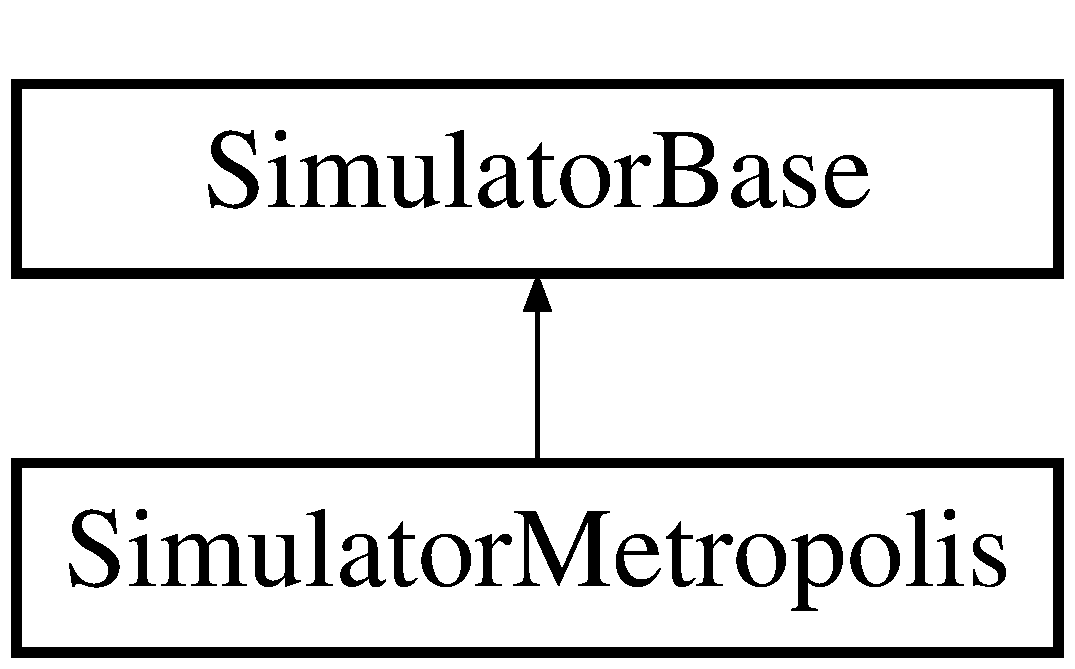
\includegraphics[height=2.000000cm]{classSimulatorMetropolis}
\end{center}
\end{figure}
\subsection*{Public Member Functions}
\begin{DoxyCompactItemize}
\item 
\mbox{\Hypertarget{classSimulatorMetropolis_ac9864831658bddb8d5ba9651c8614cbe}\label{classSimulatorMetropolis_ac9864831658bddb8d5ba9651c8614cbe}} 
void {\bfseries finish} ()
\item 
\mbox{\Hypertarget{classSimulatorMetropolis_aaf39e8c5ce23362bbb8a4f2b1cf19dda}\label{classSimulatorMetropolis_aaf39e8c5ce23362bbb8a4f2b1cf19dda}} 
void {\bfseries setup} (const \mbox{\hyperlink{classParameters}{Parameters}} \&)
\end{DoxyCompactItemize}
\subsection*{Additional Inherited Members}


The documentation for this class was generated from the following files\+:\begin{DoxyCompactItemize}
\item 
control/simulator\+Metropolis.\+hpp\item 
control/simulator\+Metropolis.\+cpp\end{DoxyCompactItemize}

\hypertarget{classSimulatorRate}{}\section{Simulator\+Rate Class Reference}
\label{classSimulatorRate}\index{Simulator\+Rate@{Simulator\+Rate}}
Inheritance diagram for Simulator\+Rate\+:\begin{figure}[H]
\begin{center}
\leavevmode
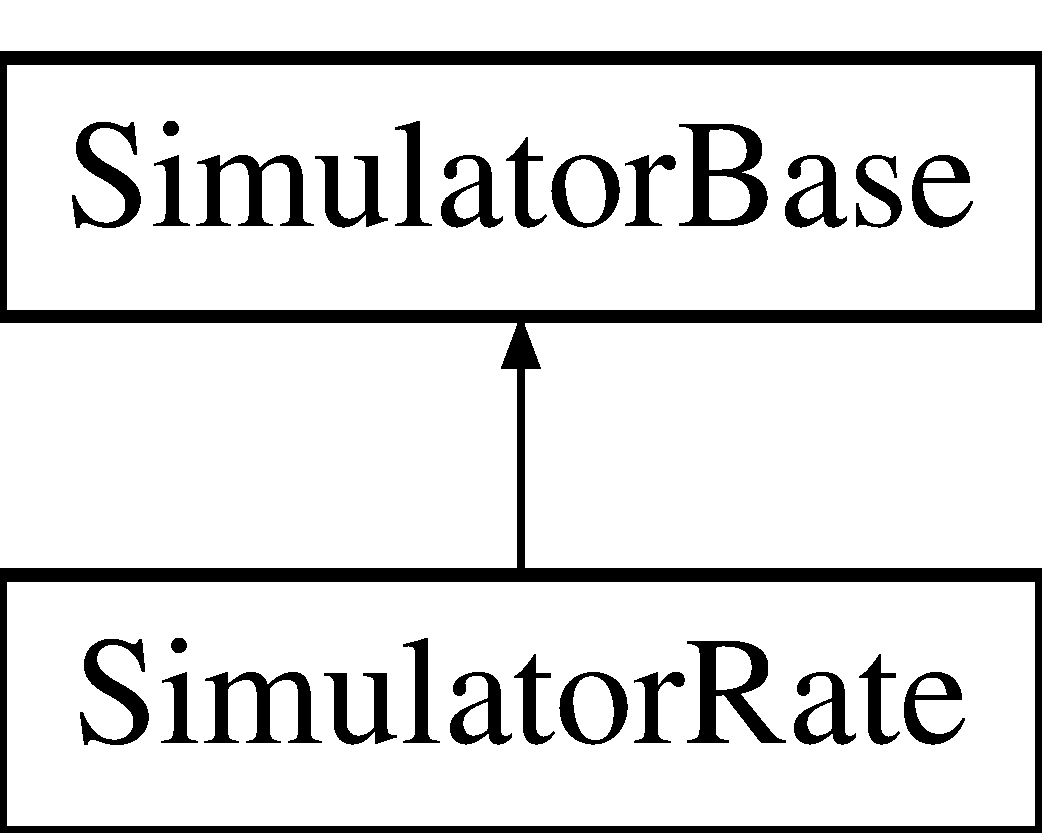
\includegraphics[height=2.000000cm]{classSimulatorRate}
\end{center}
\end{figure}
\subsection*{Public Member Functions}
\begin{DoxyCompactItemize}
\item 
\mbox{\Hypertarget{classSimulatorRate_a1d7ef6edfaa042ef54231709251fd9b4}\label{classSimulatorRate_a1d7ef6edfaa042ef54231709251fd9b4}} 
void {\bfseries finish} ()
\item 
\mbox{\Hypertarget{classSimulatorRate_a42e01c94f488c76b918e5cfbff8c7909}\label{classSimulatorRate_a42e01c94f488c76b918e5cfbff8c7909}} 
void {\bfseries setup} (const \mbox{\hyperlink{classParameters}{Parameters}} \&)
\end{DoxyCompactItemize}
\subsection*{Additional Inherited Members}


The documentation for this class was generated from the following files\+:\begin{DoxyCompactItemize}
\item 
control/simulator\+Rate.\+hpp\item 
control/simulator\+Rate.\+cpp\end{DoxyCompactItemize}

\hypertarget{classTopology}{}\section{Topology Class Reference}
\label{classTopology}\index{Topology@{Topology}}
Inheritance diagram for Topology\+:\begin{figure}[H]
\begin{center}
\leavevmode
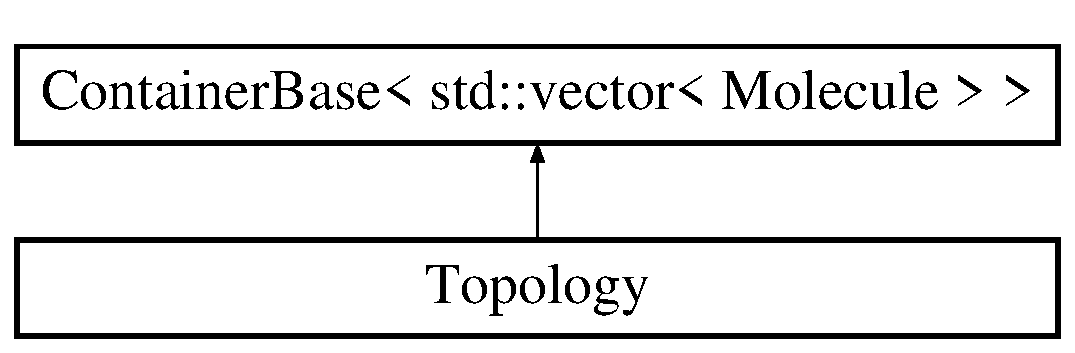
\includegraphics[height=2.000000cm]{classTopology}
\end{center}
\end{figure}
\subsection*{Public Member Functions}
\begin{DoxyCompactItemize}
\item 
\mbox{\Hypertarget{classTopology_a43e08a71c5c230a3b80a2254bb7590dd}\label{classTopology_a43e08a71c5c230a3b80a2254bb7590dd}} 
void {\bfseries set\+Dimensions} (const R\+E\+A\+L\+V\+EC \&d)
\item 
\mbox{\Hypertarget{classTopology_a00fe36f612b0f115f0c8021b846c4bf6}\label{classTopology_a00fe36f612b0f115f0c8021b846c4bf6}} 
const auto \& {\bfseries get\+Dimensions} () const
\item 
\mbox{\Hypertarget{classTopology_ae63fd2235cbe695a3d8fd447efba931d}\label{classTopology_ae63fd2235cbe695a3d8fd447efba931d}} 
void {\bfseries add\+Reaction\+Record} (const std\+::size\+\_\+t \&molid)
\item 
\mbox{\Hypertarget{classTopology_a7bb2878be1add1b4b27750966d561eae}\label{classTopology_a7bb2878be1add1b4b27750966d561eae}} 
const auto \& {\bfseries get\+Reaction\+Records\+Atoms} ()
\item 
\mbox{\Hypertarget{classTopology_a257fce4a1dd8785861a001fca1847d4e}\label{classTopology_a257fce4a1dd8785861a001fca1847d4e}} 
const auto \& {\bfseries get\+Reaction\+Records\+Molecules} ()
\item 
\mbox{\Hypertarget{classTopology_a4bca05cee9589ad00b18d92c67646bea}\label{classTopology_a4bca05cee9589ad00b18d92c67646bea}} 
const std\+::size\+\_\+t \& {\bfseries get\+Reaction\+Record\+Molecule} (const std\+::size\+\_\+t \&oldmolid)
\item 
\mbox{\Hypertarget{classTopology_a5a99967e344fd10de5c61bc4839f4681}\label{classTopology_a5a99967e344fd10de5c61bc4839f4681}} 
auto {\bfseries add\+Molecule} (\mbox{\hyperlink{classMolecule}{Molecule}} m)
\item 
\mbox{\Hypertarget{classTopology_a13905ac1030de2330788a80b3ba10adc}\label{classTopology_a13905ac1030de2330788a80b3ba10adc}} 
auto {\bfseries add\+Molecule} (std\+::size\+\_\+t id, std\+::string name)
\item 
\mbox{\Hypertarget{classTopology_adf853f3c5e1faaa520945fa4d8636cb7}\label{classTopology_adf853f3c5e1faaa520945fa4d8636cb7}} 
void {\bfseries remove\+Molecule} (\mbox{\hyperlink{classMolecule}{Molecule}} \&)
\item 
\mbox{\Hypertarget{classTopology_a43bde0718e4d50ccfd96ef7d55ee9511}\label{classTopology_a43bde0718e4d50ccfd96ef7d55ee9511}} 
void {\bfseries remove\+Molecule} (std\+::size\+\_\+t)
\item 
\mbox{\Hypertarget{classTopology_ae75e30fd331e67182af3de9f7561260a}\label{classTopology_ae75e30fd331e67182af3de9f7561260a}} 
bool {\bfseries contains\+Molecule} (const \mbox{\hyperlink{classMolecule}{Molecule}} \&) const
\item 
\mbox{\Hypertarget{classTopology_a5bffe8e0a383173f10e447c95fdaef9e}\label{classTopology_a5bffe8e0a383173f10e447c95fdaef9e}} 
bool {\bfseries contains\+Molecule} (const std\+::size\+\_\+t \&) const
\item 
\mbox{\Hypertarget{classTopology_a24590a20d20d07d4807d1e28da3c55e5}\label{classTopology_a24590a20d20d07d4807d1e28da3c55e5}} 
const \mbox{\hyperlink{classMolecule}{Molecule}} \& {\bfseries get\+Molecule} (std\+::size\+\_\+t) const
\item 
\mbox{\Hypertarget{classTopology_a9f3a2f9b847f89d5bbfd214d96391e77}\label{classTopology_a9f3a2f9b847f89d5bbfd214d96391e77}} 
std\+::vector$<$ std\+::reference\+\_\+wrapper$<$ \mbox{\hyperlink{classMolecule}{Molecule}} $>$ $>$ {\bfseries get\+Molecules} (std\+::string)
\item 
\mbox{\Hypertarget{classTopology_a53c46d18870e7610f73024504ff1ebcd}\label{classTopology_a53c46d18870e7610f73024504ff1ebcd}} 
\mbox{\hyperlink{classMolecule}{Molecule}} \& {\bfseries get\+Add\+Molecule} (std\+::size\+\_\+t, std\+::string)
\item 
\mbox{\Hypertarget{classTopology_a57508c2466292d7f42b1b446a514ab70}\label{classTopology_a57508c2466292d7f42b1b446a514ab70}} 
std\+::vector$<$ std\+::string $>$ {\bfseries get\+Moleculetypes} () const
\item 
\mbox{\Hypertarget{classTopology_ab26d60ea35ac26b9afb849e1390648e3}\label{classTopology_ab26d60ea35ac26b9afb849e1390648e3}} 
const auto {\bfseries get\+N\+Atoms} () const
\item 
\mbox{\Hypertarget{classTopology_a7f61d561ac897adf0a9735ed66fa70b5}\label{classTopology_a7f61d561ac897adf0a9735ed66fa70b5}} 
void {\bfseries sort} ()
\item 
\mbox{\Hypertarget{classTopology_a75a2d3933bc3af05e1ae0539b198d1a2}\label{classTopology_a75a2d3933bc3af05e1ae0539b198d1a2}} 
void {\bfseries repair\+Molecule\+P\+BC} (\mbox{\hyperlink{classMolecule}{Molecule}} \&)
\item 
\mbox{\Hypertarget{classTopology_a785d0b5028f6f0c2d42fbb726c4ecc2c}\label{classTopology_a785d0b5028f6f0c2d42fbb726c4ecc2c}} 
bool {\bfseries empty} () const
\item 
\mbox{\Hypertarget{classTopology_a156c05ef747fba350adc5f790a16367a}\label{classTopology_a156c05ef747fba350adc5f790a16367a}} 
void {\bfseries clear} ()
\item 
\mbox{\Hypertarget{classTopology_aa549f8bec1377e04c677c24787d412ac}\label{classTopology_aa549f8bec1377e04c677c24787d412ac}} 
void {\bfseries clear\+Reaction\+Records} ()
\end{DoxyCompactItemize}
\subsection*{Friends}
\begin{DoxyCompactItemize}
\item 
\mbox{\Hypertarget{classTopology_a6cd9eecf891bc3fcc4074b52de52c1fc}\label{classTopology_a6cd9eecf891bc3fcc4074b52de52c1fc}} 
std\+::ostream \& {\bfseries operator$<$$<$} (std\+::ostream \&os, const \mbox{\hyperlink{classTopology}{Topology}} \&obj)
\end{DoxyCompactItemize}
\subsection*{Additional Inherited Members}


The documentation for this class was generated from the following files\+:\begin{DoxyCompactItemize}
\item 
container/topology.\+hpp\item 
container/topology.\+cpp\end{DoxyCompactItemize}

\hypertarget{classTopologyParserBase}{}\section{Topology\+Parser\+Base Class Reference}
\label{classTopologyParserBase}\index{Topology\+Parser\+Base@{Topology\+Parser\+Base}}
Inheritance diagram for Topology\+Parser\+Base\+:\begin{figure}[H]
\begin{center}
\leavevmode
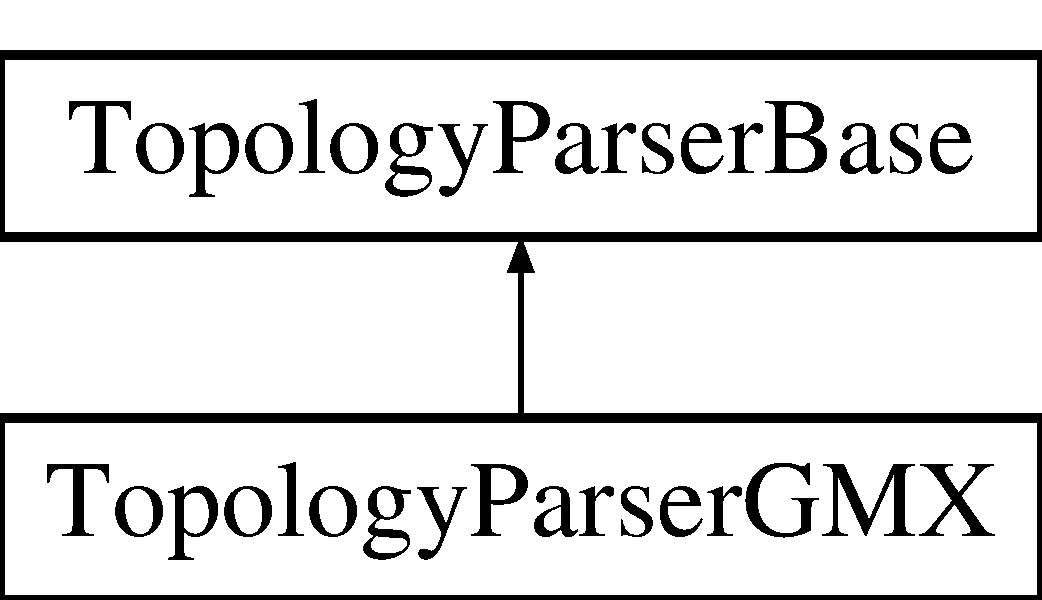
\includegraphics[height=2.000000cm]{classTopologyParserBase}
\end{center}
\end{figure}
\subsection*{Public Member Functions}
\begin{DoxyCompactItemize}
\item 
\mbox{\Hypertarget{classTopologyParserBase_ab793e27d1afb4c167112a39ed4694405}\label{classTopologyParserBase_ab793e27d1afb4c167112a39ed4694405}} 
virtual void {\bfseries read} (\mbox{\hyperlink{classTopology}{Topology}} \&, const std\+::size\+\_\+t \&)=0
\item 
\mbox{\Hypertarget{classTopologyParserBase_ad48ed8f34ef58e18db398c1aa4dd15cb}\label{classTopologyParserBase_ad48ed8f34ef58e18db398c1aa4dd15cb}} 
virtual void {\bfseries read\+Relaxed} (\mbox{\hyperlink{classTopology}{Topology}} \&, const std\+::size\+\_\+t \&)=0
\item 
\mbox{\Hypertarget{classTopologyParserBase_a7843761ed48d512c19f977c7fe1906e3}\label{classTopologyParserBase_a7843761ed48d512c19f977c7fe1906e3}} 
virtual void {\bfseries write} (\mbox{\hyperlink{classTopology}{Topology}} \&, const std\+::size\+\_\+t \&)=0
\end{DoxyCompactItemize}


The documentation for this class was generated from the following file\+:\begin{DoxyCompactItemize}
\item 
parser/topology\+Parser\+Base.\+hpp\end{DoxyCompactItemize}

\hypertarget{classTopologyParserGMX}{}\section{Topology\+Parser\+G\+MX Class Reference}
\label{classTopologyParserGMX}\index{Topology\+Parser\+G\+MX@{Topology\+Parser\+G\+MX}}
Inheritance diagram for Topology\+Parser\+G\+MX\+:\begin{figure}[H]
\begin{center}
\leavevmode
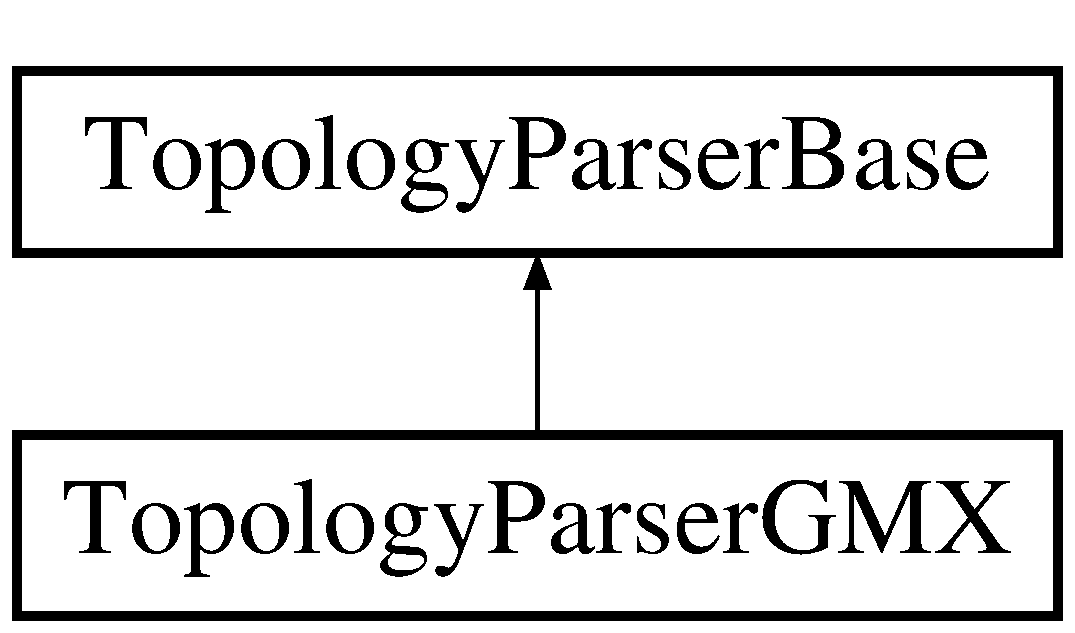
\includegraphics[height=2.000000cm]{classTopologyParserGMX}
\end{center}
\end{figure}
\subsection*{Public Member Functions}
\begin{DoxyCompactItemize}
\item 
\mbox{\Hypertarget{classTopologyParserGMX_a49fd91d03ee08c506e927281006c69ca}\label{classTopologyParserGMX_a49fd91d03ee08c506e927281006c69ca}} 
void {\bfseries read} (\mbox{\hyperlink{classTopology}{Topology}} \&, const std\+::size\+\_\+t \&)
\item 
\mbox{\Hypertarget{classTopologyParserGMX_a7c9ad910dffa3a75449d8fda1cfab443}\label{classTopologyParserGMX_a7c9ad910dffa3a75449d8fda1cfab443}} 
void {\bfseries read\+Relaxed} (\mbox{\hyperlink{classTopology}{Topology}} \&, const std\+::size\+\_\+t \&)
\item 
\mbox{\Hypertarget{classTopologyParserGMX_a499269cc13e88d86c7ce74364308214c}\label{classTopologyParserGMX_a499269cc13e88d86c7ce74364308214c}} 
void {\bfseries write} (\mbox{\hyperlink{classTopology}{Topology}} \&, const std\+::size\+\_\+t \&)
\end{DoxyCompactItemize}


The documentation for this class was generated from the following files\+:\begin{DoxyCompactItemize}
\item 
parser/topology\+Parser\+G\+M\+X.\+hpp\item 
parser/topology\+Parser\+G\+M\+X.\+cpp\end{DoxyCompactItemize}

\hypertarget{structTransitionTable}{}\section{Transition\+Table Struct Reference}
\label{structTransitionTable}\index{Transition\+Table@{Transition\+Table}}
\subsection*{Public Member Functions}
\begin{DoxyCompactItemize}
\item 
\mbox{\Hypertarget{structTransitionTable_aa2b220b550c79c7b48211c5484ae13be}\label{structTransitionTable_aa2b220b550c79c7b48211c5484ae13be}} 
{\bfseries Transition\+Table} (const std\+::size\+\_\+t \&ix1, const std\+::size\+\_\+t \&ix2, const std\+::size\+\_\+t \&ix3, const std\+::size\+\_\+t \&ix4)
\end{DoxyCompactItemize}
\subsection*{Public Attributes}
\begin{DoxyCompactItemize}
\item 
\mbox{\Hypertarget{structTransitionTable_ab91971a0da0724c383a8d18957a8a4b4}\label{structTransitionTable_ab91971a0da0724c383a8d18957a8a4b4}} 
std\+::size\+\_\+t {\bfseries old\+Molix} \{0\}
\item 
\mbox{\Hypertarget{structTransitionTable_afed5ad58c234ec2e9c028717def6eb82}\label{structTransitionTable_afed5ad58c234ec2e9c028717def6eb82}} 
std\+::size\+\_\+t {\bfseries oldix} \{0\}
\item 
\mbox{\Hypertarget{structTransitionTable_adc7b9bd91e216846e38e45db12bf1bd0}\label{structTransitionTable_adc7b9bd91e216846e38e45db12bf1bd0}} 
std\+::size\+\_\+t {\bfseries new\+Molix} \{0\}
\item 
\mbox{\Hypertarget{structTransitionTable_a309d4aec7a7d534805ecaf85d4875eef}\label{structTransitionTable_a309d4aec7a7d534805ecaf85d4875eef}} 
std\+::size\+\_\+t {\bfseries newix} \{0\}
\end{DoxyCompactItemize}


The documentation for this struct was generated from the following file\+:\begin{DoxyCompactItemize}
\item 
reaction/reaction\+Base.\+hpp\end{DoxyCompactItemize}

\hypertarget{structTranslationTable}{}\section{Translation\+Table Struct Reference}
\label{structTranslationTable}\index{Translation\+Table@{Translation\+Table}}
\subsection*{Public Member Functions}
\begin{DoxyCompactItemize}
\item 
\mbox{\Hypertarget{structTranslationTable_aeacc22b9cb61b4058ee2624e9d5f7eac}\label{structTranslationTable_aeacc22b9cb61b4058ee2624e9d5f7eac}} 
{\bfseries Translation\+Table} (const std\+::pair$<$ std\+::size\+\_\+t, std\+::size\+\_\+t $>$ \&ix1, const std\+::pair$<$ std\+::size\+\_\+t, std\+::size\+\_\+t $>$ \&ix2, const R\+E\+AL \&val)
\end{DoxyCompactItemize}
\subsection*{Public Attributes}
\begin{DoxyCompactItemize}
\item 
\mbox{\Hypertarget{structTranslationTable_aca64d8bf2021a8843cd86a8db523d943}\label{structTranslationTable_aca64d8bf2021a8843cd86a8db523d943}} 
std\+::pair$<$ std\+::size\+\_\+t, std\+::size\+\_\+t $>$ {\bfseries indices1} \{\}
\item 
\mbox{\Hypertarget{structTranslationTable_a72ff633c1eb629a9aef566762a40ea77}\label{structTranslationTable_a72ff633c1eb629a9aef566762a40ea77}} 
std\+::pair$<$ std\+::size\+\_\+t, std\+::size\+\_\+t $>$ {\bfseries indices2} \{\}
\item 
\mbox{\Hypertarget{structTranslationTable_ae7a379d21dc16132732b56653e7ec791}\label{structTranslationTable_ae7a379d21dc16132732b56653e7ec791}} 
R\+E\+AL {\bfseries value} \{0\}
\end{DoxyCompactItemize}


The documentation for this struct was generated from the following file\+:\begin{DoxyCompactItemize}
\item 
reaction/reaction\+Base.\+hpp\end{DoxyCompactItemize}

\hypertarget{classUniverse}{}\section{Universe Class Reference}
\label{classUniverse}\index{Universe@{Universe}}
\subsection*{Public Member Functions}
\begin{DoxyCompactItemize}
\item 
\mbox{\Hypertarget{classUniverse_a9e3bc4f94ef91856fed80ccb5fab0081}\label{classUniverse_a9e3bc4f94ef91856fed80ccb5fab0081}} 
void {\bfseries setup} (const \mbox{\hyperlink{classParameters}{Parameters}} \&)
\item 
\mbox{\Hypertarget{classUniverse_a6a93f69c9178fc17789afbcac9920e55}\label{classUniverse_a6a93f69c9178fc17789afbcac9920e55}} 
void {\bfseries update} (const std\+::size\+\_\+t \&)
\item 
\mbox{\Hypertarget{classUniverse_af75ed4503afd48ecf21618b0a1026bf1}\label{classUniverse_af75ed4503afd48ecf21618b0a1026bf1}} 
void {\bfseries write} (const std\+::size\+\_\+t \&)
\item 
\mbox{\Hypertarget{classUniverse_a47d6b992adc8a541cdb75605df055d43}\label{classUniverse_a47d6b992adc8a541cdb75605df055d43}} 
void {\bfseries read\+Relaxed} (const std\+::size\+\_\+t \&)
\item 
\mbox{\Hypertarget{classUniverse_a2d33d546d563a374544c0d0e9c335397}\label{classUniverse_a2d33d546d563a374544c0d0e9c335397}} 
std\+::vector$<$ \mbox{\hyperlink{classReactionCandidate}{Reaction\+Candidate}} $>$ {\bfseries search\+Reaction\+Candidates} ()
\item 
\mbox{\Hypertarget{classUniverse_a31495ec00a1acff8471f4fabf12c7b93}\label{classUniverse_a31495ec00a1acff8471f4fabf12c7b93}} 
bool {\bfseries is\+Available} (const \mbox{\hyperlink{classReactionCandidate}{Reaction\+Candidate}} \&)
\item 
\mbox{\Hypertarget{classUniverse_a453f9af0190ca4fccb44da223bd4bae4}\label{classUniverse_a453f9af0190ca4fccb44da223bd4bae4}} 
void {\bfseries react} (\mbox{\hyperlink{classReactionCandidate}{Reaction\+Candidate}} \&)
\item 
\mbox{\Hypertarget{classUniverse_a223fed1cf57eda7e2b26de524349058a}\label{classUniverse_a223fed1cf57eda7e2b26de524349058a}} 
void {\bfseries check\+Movement} (const \mbox{\hyperlink{classReactionCandidate}{Reaction\+Candidate}} \&)
\item 
\mbox{\Hypertarget{classUniverse_af9774b79ba2478354800c4e676981aa0}\label{classUniverse_af9774b79ba2478354800c4e676981aa0}} 
const auto \& {\bfseries get\+Reaction\+Templates} () const
\end{DoxyCompactItemize}


The documentation for this class was generated from the following files\+:\begin{DoxyCompactItemize}
\item 
container/universe.\+hpp\item 
container/universe.\+cpp\end{DoxyCompactItemize}

\hypertarget{classenhance_1_1Vector3d}{}\section{enhance\+:\+:Vector3d$<$ T $>$ Class Template Reference}
\label{classenhance_1_1Vector3d}\index{enhance\+::\+Vector3d$<$ T $>$@{enhance\+::\+Vector3d$<$ T $>$}}
\subsection*{Public Member Functions}
\begin{DoxyCompactItemize}
\item 
\mbox{\Hypertarget{classenhance_1_1Vector3d_a3543948b081e615391d5187771009fb3}\label{classenhance_1_1Vector3d_a3543948b081e615391d5187771009fb3}} 
{\bfseries Vector3d} (const T)
\item 
\mbox{\Hypertarget{classenhance_1_1Vector3d_aeb44c9b3730a5b683a4a5fbabb72c71c}\label{classenhance_1_1Vector3d_aeb44c9b3730a5b683a4a5fbabb72c71c}} 
{\bfseries Vector3d} (const T, const T, const T)
\item 
\mbox{\Hypertarget{classenhance_1_1Vector3d_abaf33fc8fba175c1bbf87b1f2e5e2564}\label{classenhance_1_1Vector3d_abaf33fc8fba175c1bbf87b1f2e5e2564}} 
{\bfseries Vector3d} (const \mbox{\hyperlink{classenhance_1_1Vector3d}{Vector3d}}$<$ T $>$ \&other)=default
\item 
\mbox{\Hypertarget{classenhance_1_1Vector3d_a9a1412d434ddb2a93c1213f85988c5fe}\label{classenhance_1_1Vector3d_a9a1412d434ddb2a93c1213f85988c5fe}} 
{\bfseries Vector3d} (\mbox{\hyperlink{classenhance_1_1Vector3d}{Vector3d}}$<$ T $>$ \&\&other)=default
\item 
\mbox{\Hypertarget{classenhance_1_1Vector3d_a7f9f64359509dbb370a5d2674a771f26}\label{classenhance_1_1Vector3d_a7f9f64359509dbb370a5d2674a771f26}} 
{\footnotesize template$<$typename O $>$ }\\{\bfseries Vector3d} (const \mbox{\hyperlink{classenhance_1_1Vector3d}{Vector3d}}$<$ O $>$ \&)
\item 
\mbox{\Hypertarget{classenhance_1_1Vector3d_a13390fa422869e4048d2a49209273fe2}\label{classenhance_1_1Vector3d_a13390fa422869e4048d2a49209273fe2}} 
T \& {\bfseries operator()} (std\+::size\+\_\+t i)
\item 
\mbox{\Hypertarget{classenhance_1_1Vector3d_aa201770b97b019d5c1abf69e5b1a1c49}\label{classenhance_1_1Vector3d_aa201770b97b019d5c1abf69e5b1a1c49}} 
constexpr T {\bfseries operator()} (std\+::size\+\_\+t i) const
\item 
\mbox{\Hypertarget{classenhance_1_1Vector3d_a74225e32c5ce326ec8b8295979f65524}\label{classenhance_1_1Vector3d_a74225e32c5ce326ec8b8295979f65524}} 
T \& {\bfseries operator\mbox{[}$\,$\mbox{]}} (std\+::size\+\_\+t i)
\item 
\mbox{\Hypertarget{classenhance_1_1Vector3d_a0605d2ec5d2258edb6f429a0f2ca3b3c}\label{classenhance_1_1Vector3d_a0605d2ec5d2258edb6f429a0f2ca3b3c}} 
constexpr T {\bfseries operator\mbox{[}$\,$\mbox{]}} (std\+::size\+\_\+t i) const
\item 
\mbox{\Hypertarget{classenhance_1_1Vector3d_a902095f031fd29a5cc634f29a6c5002d}\label{classenhance_1_1Vector3d_a902095f031fd29a5cc634f29a6c5002d}} 
\mbox{\hyperlink{classenhance_1_1Vector3d}{Vector3d}}$<$ T $>$ \& {\bfseries operator=} (const \mbox{\hyperlink{classenhance_1_1Vector3d}{Vector3d}}$<$ T $>$ \&)
\item 
\mbox{\Hypertarget{classenhance_1_1Vector3d_ad45050c6e7a976fedf68b2188b91c08e}\label{classenhance_1_1Vector3d_ad45050c6e7a976fedf68b2188b91c08e}} 
\mbox{\hyperlink{classenhance_1_1Vector3d}{Vector3d}}$<$ T $>$ \& {\bfseries operator=} (\mbox{\hyperlink{classenhance_1_1Vector3d}{Vector3d}}$<$ T $>$ \&\&)
\item 
\mbox{\Hypertarget{classenhance_1_1Vector3d_a8c713ef30317a14de572aef4cc2a9c32}\label{classenhance_1_1Vector3d_a8c713ef30317a14de572aef4cc2a9c32}} 
{\footnotesize template$<$typename O $>$ }\\const \mbox{\hyperlink{classenhance_1_1Vector3d}{Vector3d}}$<$ T $>$ {\bfseries operator$\ast$} (const O \&) const
\item 
\mbox{\Hypertarget{classenhance_1_1Vector3d_a83bfd54db1359389c9d22efed2c3f50f}\label{classenhance_1_1Vector3d_a83bfd54db1359389c9d22efed2c3f50f}} 
{\footnotesize template$<$typename O $>$ }\\\mbox{\hyperlink{classenhance_1_1Vector3d}{Vector3d}}$<$ T $>$ {\bfseries operator$\ast$} (O \&\&) const
\item 
\mbox{\Hypertarget{classenhance_1_1Vector3d_a911799196cd145ed67384623943659c8}\label{classenhance_1_1Vector3d_a911799196cd145ed67384623943659c8}} 
{\footnotesize template$<$typename O $>$ }\\const \mbox{\hyperlink{classenhance_1_1Vector3d}{Vector3d}}$<$ T $>$ {\bfseries operator/} (const O \&) const
\item 
\mbox{\Hypertarget{classenhance_1_1Vector3d_add3791808ae6d592cd2ead3654fd5295}\label{classenhance_1_1Vector3d_add3791808ae6d592cd2ead3654fd5295}} 
{\footnotesize template$<$typename O $>$ }\\\mbox{\hyperlink{classenhance_1_1Vector3d}{Vector3d}}$<$ T $>$ {\bfseries operator/} (O \&\&) const
\item 
\mbox{\Hypertarget{classenhance_1_1Vector3d_ab17dc155ecc52dfdaffa162882c6e679}\label{classenhance_1_1Vector3d_ab17dc155ecc52dfdaffa162882c6e679}} 
{\footnotesize template$<$typename O $>$ }\\const \mbox{\hyperlink{classenhance_1_1Vector3d}{Vector3d}}$<$ T $>$ {\bfseries operator+} (const \mbox{\hyperlink{classenhance_1_1Vector3d}{Vector3d}}$<$ O $>$ \&) const
\item 
\mbox{\Hypertarget{classenhance_1_1Vector3d_aa3bac62d54a54ee8ff03cd5e61975af2}\label{classenhance_1_1Vector3d_aa3bac62d54a54ee8ff03cd5e61975af2}} 
{\footnotesize template$<$typename O $>$ }\\\mbox{\hyperlink{classenhance_1_1Vector3d}{Vector3d}}$<$ T $>$ {\bfseries operator+} (\mbox{\hyperlink{classenhance_1_1Vector3d}{Vector3d}}$<$ O $>$ \&\&) const
\item 
\mbox{\Hypertarget{classenhance_1_1Vector3d_a11e2f814fc5525552f3f24396ac2eb60}\label{classenhance_1_1Vector3d_a11e2f814fc5525552f3f24396ac2eb60}} 
{\footnotesize template$<$typename O $>$ }\\const \mbox{\hyperlink{classenhance_1_1Vector3d}{Vector3d}}$<$ T $>$ {\bfseries operator-\/} (const \mbox{\hyperlink{classenhance_1_1Vector3d}{Vector3d}}$<$ O $>$ \&) const
\item 
\mbox{\Hypertarget{classenhance_1_1Vector3d_ada6850e861c6a2b3df35432661b900e5}\label{classenhance_1_1Vector3d_ada6850e861c6a2b3df35432661b900e5}} 
{\footnotesize template$<$typename O $>$ }\\\mbox{\hyperlink{classenhance_1_1Vector3d}{Vector3d}}$<$ T $>$ {\bfseries operator-\/} (\mbox{\hyperlink{classenhance_1_1Vector3d}{Vector3d}}$<$ O $>$ \&\&) const
\item 
\mbox{\Hypertarget{classenhance_1_1Vector3d_a0358f0479f1b1b3a1505b2da742ddecb}\label{classenhance_1_1Vector3d_a0358f0479f1b1b3a1505b2da742ddecb}} 
const \mbox{\hyperlink{classenhance_1_1Vector3d}{Vector3d}}$<$ T $>$ {\bfseries operator-\/} () const
\item 
\mbox{\Hypertarget{classenhance_1_1Vector3d_ae5e2225d3ed23344ba10a7f1756ba77b}\label{classenhance_1_1Vector3d_ae5e2225d3ed23344ba10a7f1756ba77b}} 
{\footnotesize template$<$typename O $>$ }\\\mbox{\hyperlink{classenhance_1_1Vector3d}{Vector3d}}$<$ T $>$ {\bfseries operator$\ast$=} (const O \&)
\item 
\mbox{\Hypertarget{classenhance_1_1Vector3d_a4371b92a35eceb24bfe633c36726e878}\label{classenhance_1_1Vector3d_a4371b92a35eceb24bfe633c36726e878}} 
{\footnotesize template$<$typename O $>$ }\\\mbox{\hyperlink{classenhance_1_1Vector3d}{Vector3d}}$<$ T $>$ {\bfseries operator/=} (const O \&)
\item 
\mbox{\Hypertarget{classenhance_1_1Vector3d_a7c7e17a102212918dbad00d014272399}\label{classenhance_1_1Vector3d_a7c7e17a102212918dbad00d014272399}} 
{\footnotesize template$<$typename O $>$ }\\\mbox{\hyperlink{classenhance_1_1Vector3d}{Vector3d}}$<$ T $>$ {\bfseries operator+=} (const \mbox{\hyperlink{classenhance_1_1Vector3d}{Vector3d}}$<$ O $>$ \&)
\item 
\mbox{\Hypertarget{classenhance_1_1Vector3d_af45886b1230accc137684d9c5c0b4bb5}\label{classenhance_1_1Vector3d_af45886b1230accc137684d9c5c0b4bb5}} 
{\footnotesize template$<$typename O $>$ }\\\mbox{\hyperlink{classenhance_1_1Vector3d}{Vector3d}}$<$ T $>$ {\bfseries operator-\/=} (const \mbox{\hyperlink{classenhance_1_1Vector3d}{Vector3d}}$<$ O $>$ \&)
\item 
\mbox{\Hypertarget{classenhance_1_1Vector3d_adb2099ce6415581adc90c9e4ba9ca2c5}\label{classenhance_1_1Vector3d_adb2099ce6415581adc90c9e4ba9ca2c5}} 
bool {\bfseries operator==} (const \mbox{\hyperlink{classenhance_1_1Vector3d}{Vector3d}}$<$ T $>$ \&)
\item 
\mbox{\Hypertarget{classenhance_1_1Vector3d_a8423258933d5ec4eb332eae304735b62}\label{classenhance_1_1Vector3d_a8423258933d5ec4eb332eae304735b62}} 
bool {\bfseries operator!=} (const \mbox{\hyperlink{classenhance_1_1Vector3d}{Vector3d}}$<$ T $>$ \&)
\item 
\mbox{\Hypertarget{classenhance_1_1Vector3d_a1a640f95c426d1fc38f6ae12724c3525}\label{classenhance_1_1Vector3d_a1a640f95c426d1fc38f6ae12724c3525}} 
auto {\bfseries begin} ()
\item 
\mbox{\Hypertarget{classenhance_1_1Vector3d_a1939d73182d30e43102ac97cdf33d855}\label{classenhance_1_1Vector3d_a1939d73182d30e43102ac97cdf33d855}} 
auto {\bfseries end} ()
\item 
\mbox{\Hypertarget{classenhance_1_1Vector3d_abeedf79cf94982e0f317bfe639525451}\label{classenhance_1_1Vector3d_abeedf79cf94982e0f317bfe639525451}} 
auto {\bfseries begin} () const
\item 
\mbox{\Hypertarget{classenhance_1_1Vector3d_a39871f95c19f81debcb1fc20dacd6e2b}\label{classenhance_1_1Vector3d_a39871f95c19f81debcb1fc20dacd6e2b}} 
auto {\bfseries end} () const
\item 
\mbox{\Hypertarget{classenhance_1_1Vector3d_a016878b0ff0d248197ea6d4e8ac2e931}\label{classenhance_1_1Vector3d_a016878b0ff0d248197ea6d4e8ac2e931}} 
auto {\bfseries cbegin} () const
\item 
\mbox{\Hypertarget{classenhance_1_1Vector3d_ad62c9df3053fb3556ace45bb5b1c2c0e}\label{classenhance_1_1Vector3d_ad62c9df3053fb3556ace45bb5b1c2c0e}} 
auto {\bfseries cend} () const
\item 
\mbox{\Hypertarget{classenhance_1_1Vector3d_a1c1d6cd87f4cb8c4dcead3923575a57d}\label{classenhance_1_1Vector3d_a1c1d6cd87f4cb8c4dcead3923575a57d}} 
auto {\bfseries rbegin} ()
\item 
\mbox{\Hypertarget{classenhance_1_1Vector3d_a6a97f9a75cfde7d24657f24e5b04556c}\label{classenhance_1_1Vector3d_a6a97f9a75cfde7d24657f24e5b04556c}} 
auto {\bfseries rend} ()
\item 
\mbox{\Hypertarget{classenhance_1_1Vector3d_a076eef19933c1e90237ce466511b867c}\label{classenhance_1_1Vector3d_a076eef19933c1e90237ce466511b867c}} 
auto {\bfseries rbegin} () const
\item 
\mbox{\Hypertarget{classenhance_1_1Vector3d_ad66092240cc90be5d9539e082af96298}\label{classenhance_1_1Vector3d_ad66092240cc90be5d9539e082af96298}} 
auto {\bfseries rend} () const
\item 
\mbox{\Hypertarget{classenhance_1_1Vector3d_a06ab8677208966dacba935db0fbdecfb}\label{classenhance_1_1Vector3d_a06ab8677208966dacba935db0fbdecfb}} 
auto {\bfseries crbegin} () const
\item 
\mbox{\Hypertarget{classenhance_1_1Vector3d_a74beabb38c536d232db01529ab4c872d}\label{classenhance_1_1Vector3d_a74beabb38c536d232db01529ab4c872d}} 
auto {\bfseries crend} () const
\item 
\mbox{\Hypertarget{classenhance_1_1Vector3d_a3fcb5baa3320c241e8e07d1bcff235af}\label{classenhance_1_1Vector3d_a3fcb5baa3320c241e8e07d1bcff235af}} 
float {\bfseries norm} () const
\item 
\mbox{\Hypertarget{classenhance_1_1Vector3d_a776ae8af961aa74c79f9daa254f19bf6}\label{classenhance_1_1Vector3d_a776ae8af961aa74c79f9daa254f19bf6}} 
{\footnotesize template$<$typename O $>$ }\\T {\bfseries dot} (const \mbox{\hyperlink{classenhance_1_1Vector3d}{Vector3d}}$<$ O $>$ \&) const
\item 
\mbox{\Hypertarget{classenhance_1_1Vector3d_adf1041d6815b6d3c304866309b246461}\label{classenhance_1_1Vector3d_adf1041d6815b6d3c304866309b246461}} 
{\footnotesize template$<$typename O $>$ }\\\mbox{\hyperlink{classenhance_1_1Vector3d}{Vector3d}}$<$ T $>$ {\bfseries cross} (const \mbox{\hyperlink{classenhance_1_1Vector3d}{Vector3d}}$<$ O $>$ \&) const
\item 
\mbox{\Hypertarget{classenhance_1_1Vector3d_a19492f5b72c825f70d0aba9756c3f975}\label{classenhance_1_1Vector3d_a19492f5b72c825f70d0aba9756c3f975}} 
void {\bfseries set\+Zero} ()
\item 
\mbox{\Hypertarget{classenhance_1_1Vector3d_aded32944fc5b42b51b6bb36e5ea4a73a}\label{classenhance_1_1Vector3d_aded32944fc5b42b51b6bb36e5ea4a73a}} 
bool {\bfseries is\+Zero} () const
\end{DoxyCompactItemize}
\subsection*{Protected Attributes}
\begin{DoxyCompactItemize}
\item 
\mbox{\Hypertarget{classenhance_1_1Vector3d_a6e216e575ab780dfae8a65a945ec286e}\label{classenhance_1_1Vector3d_a6e216e575ab780dfae8a65a945ec286e}} 
std\+::array$<$ T, 3 $>$ {\bfseries data}
\end{DoxyCompactItemize}
\subsection*{Friends}
\begin{DoxyCompactItemize}
\item 
\mbox{\Hypertarget{classenhance_1_1Vector3d_a6f5e8062a1500764d2b38787f1471b65}\label{classenhance_1_1Vector3d_a6f5e8062a1500764d2b38787f1471b65}} 
{\footnotesize template$<$typename O $>$ }\\\mbox{\hyperlink{classenhance_1_1Vector3d}{Vector3d}}$<$ T $>$ {\bfseries operator$\ast$} (O scalar, \mbox{\hyperlink{classenhance_1_1Vector3d}{Vector3d}}$<$ T $>$ vector)
\item 
\mbox{\Hypertarget{classenhance_1_1Vector3d_afbaa27f45fba698f24a7643be7df5dbf}\label{classenhance_1_1Vector3d_afbaa27f45fba698f24a7643be7df5dbf}} 
std\+::ostream \& {\bfseries operator$<$$<$} (std\+::ostream \&os, const \mbox{\hyperlink{classenhance_1_1Vector3d}{Vector3d}}$<$ T $>$ \&vec)
\end{DoxyCompactItemize}


The documentation for this class was generated from the following file\+:\begin{DoxyCompactItemize}
\item 
enhance/vector3d.\+hpp\end{DoxyCompactItemize}

%--- End generated contents ---

% Index
\backmatter
\newpage
\phantomsection
\clearemptydoublepage
\addcontentsline{toc}{chapter}{Index}
\printindex

\end{document}
